\documentclass[11pt, a4paper]{article}
\usepackage[english, science, small]{ku-frontpage}
\usepackage[utf8]{inputenc}
\usepackage[cache=false]{minted}
\usepackage{caption}
\usepackage{subcaption}
\usepackage[linesnumbered,ruled]{algorithm2e}
\usepackage{algpseudocode}
\usepackage{gensymb}

% Math stuff
\usepackage{amsmath,amssymb,mathtools,bm,etoolbox,stmaryrd}
% verctor command. Usage: \colvec{5}{a}{b}{c}{d}{e}
\newcount\colveccount
\newcommand*\colvec[1]{
	\global\colveccount#1
	\begin{pmatrix}
		\colvecnext
	}
	\def\colvecnext#1{
		#1
		\global\advance\colveccount-1
		\ifnum\colveccount>0
		\\
		\expandafter\colvecnext
		\else
	\end{pmatrix}
	\fi
}

% que dymbol, textmode
\newcommand*{\qed}{\hfill\ensuremath{\square}}%

% TOC properties
\setlength\arraycolsep{2 pt}
\setcounter{tocdepth}{2}
\setcounter{secnumdepth}{2}

\author{Per Steffen Czolbe (wjq874) \& Asger Hans Skovbjerg Christensen (tzw174)}
\title{Reinforcement Learning with LEGO Mindstorms}
\subtitle{Project Report}
\date{Handed in: \today}

\begin{document}
	\maketitle
	
	\section{Abstract}
	With the growing popularity of machine learning and AI, and its increasing influence on peoples daily lives, it is important to educate the general public, starting at a young age, about methods and concepts used in these applications. We explore the consumer and education oriented robotic platform LEGO Mindstorms to playfully demonstrate concepts of machine learning. This approach allows to demonstrate both physically and visually how machines learn, and gives examples of what robots are capable of achieving with machine learning. Three robots are designed to interactively demonstrate data entry, visualization, prediction and reinforcement learning concepts. We create a colour robot, which demonstrates how machines perform predictions with visual aids. A one-handed crawl robot, which learns to crawl in 20 minutes using tabular Q-learning. A swing robot, which learns to swing after five to eight hours of unsupervised continuous reinforcement learning. Videos of the results are available at \footnote{Crawl robot training montage video available at \url{https://youtu.be/NUTv-oNWEYo}.} \footnote{Swing robot video available at \url{https://youtu.be/6yY9P5vG-nA}.}.
	
	\tableofcontents
	
	
	\section{Introduction}
	
	
	Machine learning is growing in interest, and is getting wildly popular. Google trends show an almost four times increase in searches for "machine learning" over the last five years \cite{googletrendsML}, and many online sites and universities are offering courses on it. It's being used in decision making in official and private institutions, for translation and even to develop self-driving cars. Such a large influence on our daily lives means that the general public should have a basic understanding of how machine learning systems operate. To increase awareness and inform the general public about often abstract machine learning concepts, it is helpful to demonstrate the concepts in a playful and interactive way.
	
	\medskip
	
	The term "Machine Learning" refers to a collection of algorithmic and statistical models, as well as related data handling methods, and deals with many classical statistical problems, such as regression and classification, using more automated model approaches, relying on computers and algorithms for optimization and model improvement. It shares many methods and ideas with statistics, enough that they could be argued to be part of the same field \cite{jordan}.
	
	\medskip
	
	Most machine learning resources are available at the university level, which increases the barrier of entry and makes even basic concepts of machine learning inaccessible to the general public. A wider outreach and understanding of machine learning can benefit both the public and academia. A better informed public allows individuals to be able to engage in a meaningful political discussion regarding automation, laws and rules regarding data, applications and results of such systems. It could satisfy the growing popularity, as well as generate more interest in and funding for machine learning in industry and academia. 
	\medskip
	
	A platform that is often used as an educational aid to inspire children of different age groups and create an interest in STEM (Science, Technology, Engineering and Maths) is `LEGO MINDSTORMS' \cite{LEGOeducation}. This platform combines robotics and programming with the well know LEGO brick system, and allows users to playfully explore many aspects of STEM. The platform is marketed towards private enthusiasts, which form a large community of hobby engineers online, and educational facilities such as public schools and universities. LEGO collaborates directly with schools, helps teachers design their class and offers frequent competitions that student groups can compete in \cite{naerheden}. Recently, LEGO explores ways to incorporate machine learning, specifically reinforcement learning, into their educational product offering. Inspiration stems from videos of enthusiasts, who had used reinforcement learning with their LEGO Mindstorms robots to teach them to perform actions \cite{youtube_crawl}\cite{youtube_swing}. Reinforcement learning is a subject of machine learning that concerns itself with how an actor should act in an environment. In reinforcement learning, an actor learns form the consequences of its actions, rather than explicit targets, making choices based on a combination of past experiences and exploration of new choices \cite{woergoetter_porr}.
	
	\medskip
	
	In this project we explore in which ways machine learning and reinforcement learning methods could be implemented in practice, using the LEGO Mindstorms robots. We intend to built robots and implement reinforcement learning algorithms on them, or create visualizations of training and prediction of models using them. We hope to explore the complexity of this task, as well as the width of the subject both for future studies and for educational use. Each robot will be designed with a goal in mind, to learn some task and possibly visualize it, and they will cover a wide variety of methods.
	
	We approach this project by first performing a survey of the newest version of the LEGO Mindstorms platform, called EV3. Next, we then give an overview over the setup used during development. Experiment with the various motors and sensors of the system are designed to determine their accuracy and best modes of usage. This provides us with the required knowledge to dive further into the design of specific robots. Finally we present three different robots: a colour detection robot, that is able to scan optical data, visualize it and perform predictions. A Crawl robot is designed as an interactive way of experiencing how a machine learning algorithm learns. Finally, a swing robot learns how to sway back and forth on a swing by moving his legs.
	
	The code for the project is implemented in the language Python, using Jupyter notebooks, and can be found on GitHub\footnote{\texttt{https://github.com/SteffenCzolbe/LEGO-machine-learning}}. The physical construction of the robots is documented with images in the report, as well as more detailed images and videos available in the repository and on the video sharing platform YouTube.
	
	\section{EV3 System}
	The EV3 system is the third version of the LEGO Mindstorm family of robot toys. It contains a central processing component, called ''Brick``, to which motors, sensors and other peripheral devices can be attached. All components are embedded into plastic casings, which make them compatible with other LEGO parts. The LEGO Group markets the EV3 system to educational facilities and private persons in a package with build instructions and parts for multiple robots. The current product offering consists of two different packages to build a total of nine robots, including the self-balancing two wheeled ``Gyroboy'' and a sorting machine that orders LEGO bricks based on their colour. The playful development of further robots by end users is encouraged. A large community of engaged hobby robot builders has formed around the EV3 platform.
	
	This section examines the components, motors, sensors and software of the EV3 ecosystem. We combine these components later on to build our own robots.
	
	\subsection{Central component: The Brick}
	The Brick is the central processing component of each EV3 robot. It can be controlled via multiple buttons, features a small LCD screen and can be connected to a computer via Wifi, Bluetooth or USB. For peripherals, up to four motors and four Sensors can be connected. The specifications of the embedded system are seen in Table \ref{tab:EV3_dev_toolkit}.
	
	\begin{table}[H]
		\centering
		\begin{tabular}{ll}
			CPU & 32bit, 300MHz ARM9 Processor \\
			Memory & 64Mb DDR RAM\\
			Storage & 16Mb Flash, up to 32Gb SD-Card \\
			Communication & USB, Bluetooth, Wifi \\
			Peripherals & four motors, four Sensors
			
		\end{tabular}
		\caption{Specifications of the embedded system in the EV3 toolkit \cite{ev3_dev_toolkit}.}
		\label{tab:EV3_dev_toolkit}
	\end{table}
	
	
	\subsection{Motors}
	The LEGO product line includes a variety of 9V DC electrical motors, which can be used to power a wide range of LEGO models, such as cars, trains and robots. The current product offering consists of two main families: ``Power Functions'' motors and ``EV3'' servo motors. 
	\medskip
	
	The EV3 robot kit contains a medium and two large servo motors. The EV3 motors use tacho feedback to measure their alignment and rotation, which allows for more precise control compared to ``Power Functions'' motors \cite{Servo_Motor}. In strength and speed they are comparable to their ``Power Functions'' counterparts. The large EV3 motor is roughly twice as powerful as the medium one, and comes in a bigger case with different mounting points. Detailed comparisons of the mechanical and electrical properties of all LEGO motors is available at \cite{motor_comparison}.
	
	Adapters for the power cables are required to use the ``Power Functions'' motors in combination with the EV3 platform \cite{power_fun}, so since they have no significant advantages over EV3 motors, they are disregarded.
	\medskip
	
	The ev3dev programming environment offers functions for low level interactions with the EV3 motors. Available are methods to start and stop the motor, reading the angle, setting the speed and three different stopping patterns (coast, brake and hold). The medium and large EV3 Motor offer identical programming interfaces. For angle measurements, the motor saves the rotation at system start as zero degrees. During operation, the current rotation angle offset to the starting point can be read by the motor \cite{ev3_python}.
	
	\subsection{Sensors}
	While motors make the robot move, sensors are used to observe the environment and deliver a base for making decisions. In this section we provide an overview over the sensors used for this project.
	
	\subsubsection*{Button}
	One of the simplest sensors of the EV3 system is the button. It is a box-shaped sensor, where one side has a spring loaded retractable surface. This surface is the button. The sensor has two states: pushed and not pushed. Buttons are often used as an event triggers, were a push of the button starts a programmed action.
	
	\subsubsection*{Colour Sensor}
	The EV3 colour sensor works by shining red, green, blue or all three colours of light and measuring values of the reflections. The sensor can measure colours, ambient light and reflected light. When retrieving colours, the sensor cycles all three LEDS rapidly, when retrieving reflected light, only the red led is on, and when retrieving ambient light, only the blue led is on \cite{colour_sensor_python}. The colour sensor has a built-in list of possible colours, and can measure and predict white, blue, black, green, red, yellow, brown and no colour. Since the sensor measures reflection, pointing it into the air will measure (close to) (0,0,0) which it categorises as no colour.
	
	\subsubsection*{Ultrasonic Sensor}
	The EV3 Ultrasonic Sensor generates sound waves and reads their echoes to detect and measure distance from objects. It can also send single sound waves to work as sonar or listen for a sound wave that triggers the start of a program. Distances mesured range from 0-250cm. While the Python bindings of this sensor return a distance measurement with an accuracy of up to 1mm \cite{ev3_python}, LEGO advertises an accuracy of  ``up to +/-1cm'' \cite{ultraosnic_sensor}.
	
	
	\subsubsection*{Gyroscope} \label{gyro_section}
	The gyroscope sensor detects rotational motion in the plane. This can be used to measure motion of a robot. Applications are self-balancing robots, or measuring the angle of a turn of a driving robot.
	
	The gyroscope sensor measures angular acceleration with a sample rate of 1kHz. By taking the integral of the acceleration, it is able to approximate angles \cite{gyroscope}. Since the gyroscope relies on calibration and its angle measurements are an approximation, they are often highly unreliable. We discuss ways of dealing with this in the calibration and accuracy section.
	
	
	\subsection{Software}
	The EV3 platform is sold with a software system centred around LEGO's own proprietary graphical programming language based on LabVIEW. The programming language with a graphical interface enables people with limited programming experience to quickly develop simple programs that can be executed on the Brick. The graphical language is supported by an editor available as a program for Windows and Mac, and as an app for Android and iOS.
	
	While the default software is well supported by the editor and operating system of the brick, more experienced programmers might prefer a more capable language. Multiple community driven software packages exist for this purpose. These support languages such as MATLAB, Python, Java, JavaScript, C++, C, GO, Ruby, Perl, R, Lua, even direct control of the robot via command line is possible \cite{ev3dev}. For educational purposes, programs such as Scratch and Open Roberta might be relevant. Scratch is a block-based visual programming language designed especially for kids aged 8-16 \cite{scratch}, and Open Roberta is similar \cite{roberta}, focusing especially on robots. Both languages work directly with LEGO Mindstorms. We discuss our specific development set up in the next section.
	
	
	
	\section{Development Setup}
	In this section we present the development set up chosen for this project. It consists of the open source operating system ev3dev to power the brick, the ev3dev Python library to control motors and sensors, and remote procedure calls to communicate with the robot from a host computer via Jupyter notebooks.
	
	\subsection{Ev3dev Platform}
	Ev3dev is a Debian Linux-based operating system that runs on several LEGO Mindstorms compatible platforms including the LEGO Mindstorms EV3 and Raspberry Pi-powered BrickPi. It is maintained by a community of enthusiasts and offers libraries to interact with LEGO Mindstorms motors and sensors in many programming languages, such as Java, Ruby and Python \cite{ev3dev}. The Linux disk image can be downloaded at \href{https://www.ev3dev.org/}{www.ev3dev.org} and flashed on an SD card. Once the SD card is inserted into the LEGO Mindstorms brick, the brick will boot into the ev3dev operating system. A set up guide with detailed explanations on installation and guides on how to get started with development are available at the ev3dev website.
	
	\subsection{Control by external Computer}
	While the brick, after flashed with the ev3dev image, runs a Debian Linux system that can execute general purpose programs, the processing and memory constraints imposed by the hardware limit the complexity of programs executed on the brick severely. Installing a Python package takes two minutes. Executing more computationally expensive tasks like deep learning or real time video processing on the brick is not feasible.
	
	To circumvent these problems, a setup of the main program running on a computer and interacting with the brick to move motors or read sensor data has been employed by multiple community projects, such as this rubics cube solver \cite{ev3_rubics}. We follow the design approach pioneered by these projects. The brick runs a remote procedure call server, implemented by the Python3 library \texttt{rpyc}. This allows a host computer to connect to the brick and remotely interact with motors and sensors. All program logic is executed on the computer, the brick is listening to commands. Next to the performance improvements, another benefit is that the program can be executed in a Jupyter notebook on the computer, which allows to better integrate documentation and visualization into the development process.
	
	\section{Accuracy and Calibration}
	To build models that can demonstrate reinforcement learning reliably, we need accurate and reproducible sensor measurements and motor movements. We design experiments to measure the time delay and accuracy of sensors and motors. We empirically determine which ways of controlling the motors yields the most reliable outcomes, and discuss which sensors need to be calibrated before use. 
	
	\subsection{Time Delays}
	
	We tested the response time of the motors, buttons and the colour sensor, to get an understanding of how quickly we would be able to react, as well as how reliable this connection was. \footnote{The code for this can be found commented in \texttt{experiments/Response\_speed\_experiment.ipynb}.}. 
	
	For the button, a single button was connected, and we measured the time until the robot noticed that the button wasn't pressed, and repeated, this setup was very simple and was repeated 1000 times taking 19s. Mean button response was $0.019$s with a very low variance at $4.8\cdot 10^{-6}$s$^2$.
	
	Motor reaction speed was tested with a slightly more complicated setup, in which a large motor had an arm attached, that had to move to hit a button. The arm was positioned right in front of the button, such that any amount of movement would set off the button, and it would reset position after each round. A video of this setup can be found in the notebook. Motor response testing was repeated 1000 times, and took 85s. Since the time involved a button delay, a value without this was calculated by substracting the button delay mean. The mean of the new motor-only delay was $0.066$ seconds and the motor had much higher variance than the button at $3.6\cdot 10^{-4}$ seconds$^2$ and a $95\%$ percentile of $0.124$ seconds. This is also clearly visible in Figure \ref{fig:responsetimemotorbutt}.
	
	\begin{figure}[H]
		\centering
		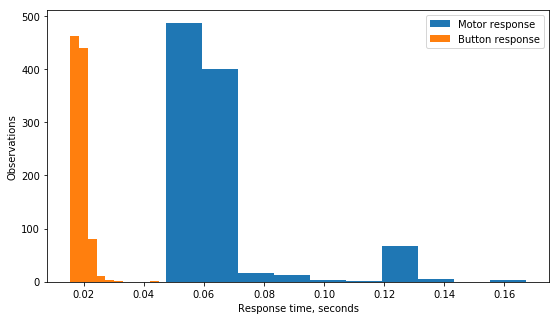
\includegraphics[width=0.6\linewidth]{images/motor_button_response_histogram.png}	
		\caption{Histogram of  response times from buttons and motors.}
		\label{fig:responsetimemotorbutt}
	\end{figure} 
	From this it appears that motor response is not only slower, but also a bit more unstable than the button response. Note though, that more factors, such as speed and real-world interference could have affected the motor response speed experiment. Still, even if assuming the 95\% percentile, we should be able to get at least eight actions per second. 
	
	The colour sensor turned out to react significantly slower than the button, probably due to the fact that it has to cycle between different LEDs. An experiment was made in which a colour sensor made an RGB observation and the time this took was logged. It was compared to an experiment in which it observed both RGB, reflected light and ambient light. Both were run 10.000 times, taking 10 and 38 minutes respectively.
	
	\begin{figure}[H]
		\centering
		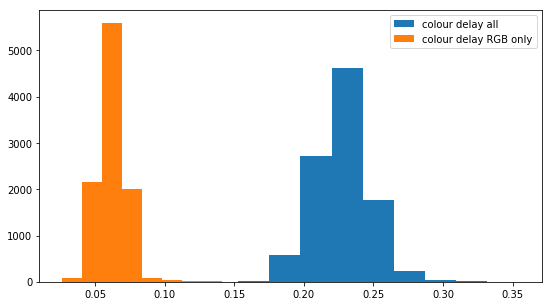
\includegraphics[width=0.6\linewidth]{images/colour_response_histogram.png} 	
		\caption{Histogram of  response times from the colour sensor if requesting only RGB colours, and if ambient and reflected light is also requested.}
		\label{fig:responsetimecolour}
	\end{figure}
	With only RGB, we observed a mean response time of $0.062$ seconds, which is very comparable to the motor response time, but with a lower variance at $1.1\cdot 10^{-4}$. With everything, the mean response was $0.228$ seconds and a variance of $3.8 \cdot 10^{-4}$. The distribution of these response times can be seen in Figure \ref{fig:responsetimecolour}, from which it seems that the response times are at least low variance.
	
	It might be possible to reduce the delay by storing information on the brick such that the transfer between brick and computer only happens once, but since the connection delay is at most $0.012$s (as evident from the button delay), the delay would still be significantly longer than RGB only. This is later used as an argument for not including ambient and reflected light as parameters in a model to be able to run in real time.
	
	\subsection{Calibration} \label{calibration}
	Servo motors and gyroscope sensors are initialized when the brick is restarted, the colour sensor has a built-in white value which can be recalibrated. All other sensors require no calibration.
	
	On system start, the position of the motor is initialized as zero degrees. If the robot is dependent on absolute positional values, it is important to calibrate the zero-point. This can either be done by moving the motor forcefully into the correct position before starting the brick, or using more elaborate constructions of moving the motor against a button, until the button is pressed. This gives certainty over the zero-position of the motor and can be used to calibrate the rotation.
	
	The gyroscope initializes its orientation at system start as zero degrees. Further, it assumes to be not in motion during system start. All acceleration measurements are in relation to this value taken during system start. Since the rotational angle returned by the gyroscope is calculated as the integral over acceleration measurements, even a slight inaccuracy in acceleration will accumulate to a significant drift in angle over time. This drift has to be monitored and adjusted for. This can be done either programmatic, or by restarting the system to re-calibrate the sensor.
	
	The colour sensor can be re-calibrated to a new relative white, but this is only used for normalization of observed colour values (originally from 0-1020) to the RGB scale. If not recalibrated, the sensor uses 300 as the maximal expected white value.
	
	
	\subsection{Motor Accuracy}
	Reinforcement learning algorithms rely on repetition of the same motions many times. To assume a non-adversarial environment and ensure reproducible results, actions taken by the motors need to be accurate and consistent. We design an experiment to measure the accuracy of the motors after a series of repeated actions.
	
	\subsubsection*{Experimental Setup}
	The experiment consists of an arm attached to a motor. We rotate the arm in a 90 degree angle back and forth. After every 25 iterations we measure the offset from the starting position externally with a set square. To measure the influence of weight on the results we use two independent arms, one without a weight and the other one weighted by three heavy metals balls. The experimental set-up is shown in Figure \ref{fig:angle_experiment}.
	
	\begin{figure}[H]
		\centering
		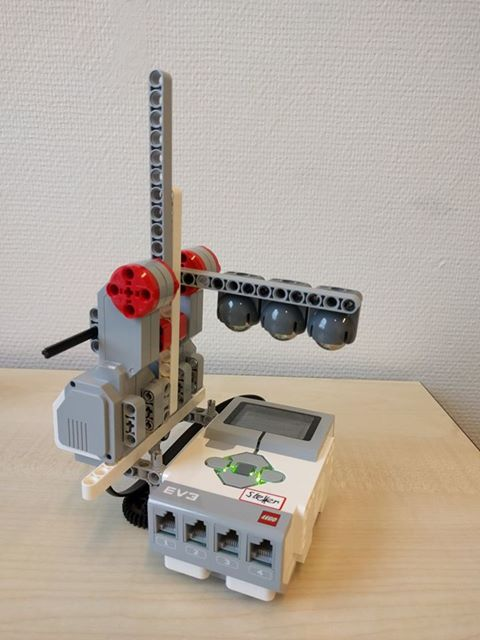
\includegraphics[width=0.35\linewidth]{images/angle_experiment}
		\caption{Experiment to measure motor accuracy. The two arms (gray) swing back and forth in a 90 degree angle. One arm is weighted down by three heavy metal balls.}
		\label{fig:angle_experiment}
	\end{figure}
	
	
	
	The ev3dev Python bindings offer two different movement patterns: \texttt{'on\_for\_degrees()'}, which rotates the motor relative to the current position, and \texttt{'move\_to\_pos()'}, which rotates the motors to an absolute value.  Further, three stopping patterns exists: \texttt{'brake'}, \texttt{'hold'} and \texttt{'coast'}. In the experiment we will test different combinations of movement and holding patterns, to determine the configuration with the highest amount of accuracy and reproducibility. Since we want high accuracy, we do not test the \texttt{'coast'} setting. The coasting option allows the motors to 'coast' until standstill, instead of enforcing them to stop at a specific position. 
	
	
	\begin{table}[H]
		\centering
		\begin{tabular}{|l|l|l|l|l|l|l|}
			\hline
			Move Pattern & Stop Pattern & Weight & inaccuracy after 25 iterations & after 50it & after 75it             & after 100it            \\ \hline \hline
			relative   & hold         & no     & 1\degree             & 1\degree    & 2\degree                & 2\degree                \\ \hline
			relative   & hold         & yes    & 9\degree             & 11\degree   & 35\degree               & 45\degree               \\ \hline
			relative   & brake        & no     & 1\degree             & 1\degree    & 1\degree                & 2\degree                \\ \hline
			relative   & brake        & yes    & 35\degree            & 50\degree   & \textgreater{}50\degree & \textgreater{}50\degree \\ \hline
			absolute     & hold         & no     & 0\degree             & 1\degree    & 2\degree                & 1\degree                \\ \hline
			absolute     & hold         & yes    & 2\degree             & 1\degree    & 4\degree                & 3\degree                \\ \hline
			absolute     & brake        & no     & 1\degree             & 2\degree    & 2\degree                & 3\degree                \\ \hline
			absolute     & brake        & yes    & 4\degree             & 6\degree    & 5\degree                & 4\degree                \\ \hline
		\end{tabular}
		\caption{Experimental result. Angle offset in degrees after 25, 50, 75 and 100 iterations for different configurations.}
		\label{tab:angle_experiment}
	\end{table}
	
	
	\subsubsection*{Results}
	The angle offsets measured after 25, 50, 75 and 100 iterations for different motor control settings and configurations are shown in table \ref{fig:angle_experiment}. As we can see, the non-weighted arm is very accurate in all scenarios. The results for the weighted arm differ drastically between configurations. We can observe two trends:
	\begin{enumerate}
		\item The \texttt{'brake'} stopping pattern creates more offset than the \texttt{'hold'} pattern. Further observations of the experiment let us conclude that \texttt{'brake'} stops the motion of the motor, but does not block the motor for further movement after the initial momentum has been eliminated. This leads to the weighted arm pulling slightly further down between the breaking phase and the next swing of the arm. The \texttt{'hold'} stop motion holds the arm in place even after the initial momentum is eliminated. It leads to more accurate results under load.
		\item Movements to absolute positions are more precise than relative movements. While inaccuracies of relative movements accumulate over time, movements to absolute positions only carry the inaccuracy of the last movement.
	\end{enumerate}
	During the experiment we also measured the range of motion that is possible without receiving any push-back from the motors. This amount of slack is consistently measured at about 12 degrees. No configuration lowered this inaccuracy. If it causes a problem later on, mechanical solutions such as a worm gear could be used to reduce the slack.
	
	\bigskip
	In conclusion, to attain the highest level of accuracy and reproducibility, motors should be moved to absolute positions and the stop pattern \texttt{'hold'} should be used. We note however that motors still allow for free movement of about 12 degrees without providing any breaking or pushback.
	
	\subsection{Ultrasonic Sensor Accuracy}
	While working with the ultrasonic sensor on the crawling robot, we noticed the importance of mounting the sensor on a stable frame. It should not tilt vertically or horizontally, as any change in angles also changes the distance to a target. To attain accurate and reliable distance measurements, the target should be a rather large, solid plane, oriented orthogonal to the ultrasonic waves emitted by the sensor. The accuracy is sufficient to measure sub-centimetre movements. Roughly 0.1\% of measurements were faulty and reported the maximum distance value of 255cm. No further experiments to evaluate the accuracy of the ultrasonic sensor have been performed.
	
	
	\subsection{Gyroscope Accuracy}
	A common complain about the EV3 system is the unreliability of the gyroscope sensor. Users commonly report issues with a 'drift' of measurements, where a non-moving sensor reports a constant non-zero speed, and angle measurements that shift over time \cite{gyro_inaccurate}. It appears that without any extra steps, the gyroscope sensor is the most unreliable out of all sensors available for the EV3 platform.
	
	To understand the drift in angle measurements, we have to understand how the gyroscope works. The gyroscope measures angular acceleration, and based on the acceleration measurements, it calculates the first integral to approximate speed, and the second integral to approximate a position or angle. When initializing, the sensor assumes to be standing still. Thus the acceleration level measured at system start is assumed to be no acceleration. If there is a slight inaccuracy, the speed and angle approximations accumulate errors over time. To reduce the drift, it is important to calibrate the sensor very accurately, for example by ensuring there is no motion in the system when it is powered on. However, the drift can not be eliminated completely. Even highly accurate gyroscopes, as used for example in space exploration, experience a drift an angle measurements by about one degree a year. In consumer goods, the drift is more significant, with mobile phones commonly experiencing drift of over one degree a minute \cite{gyro_drift}. To account for this drift, it is important to re-calibrate the sensor frequently.
	
	The sensor measures \texttt{angle} and \texttt{rate}, where \texttt{rate} describes the rate of angle change in degrees per second. When correctly calibrated, the drift can be very low. We created an experiment to check the drift over time, and to see how to calibrate the sensor for the lowest possible drift. In this experiment we attach the gyroscope to a pendulum of $30$cm length and raise the pendulum to an angle of approx 60 degrees. We release the pendulum and plot measurements taken during the swinging motion. We observed that a gyroscope reset when completely still, and routinely reset, bore the lowest drift. The result of a proper calibration is seen in Figure \ref{fig:pendulum}. We can observe that the angle, plotted in blue, forms a declining sinus form, as the pendulum swings back and forth. In orange we see the acceleration, which by manual inspection seems to be roughly the first derivative of the angle measurements, as we would expect. We see no or barely any drift in this timeframe.
	
	\begin{figure}[H]
		\centering
		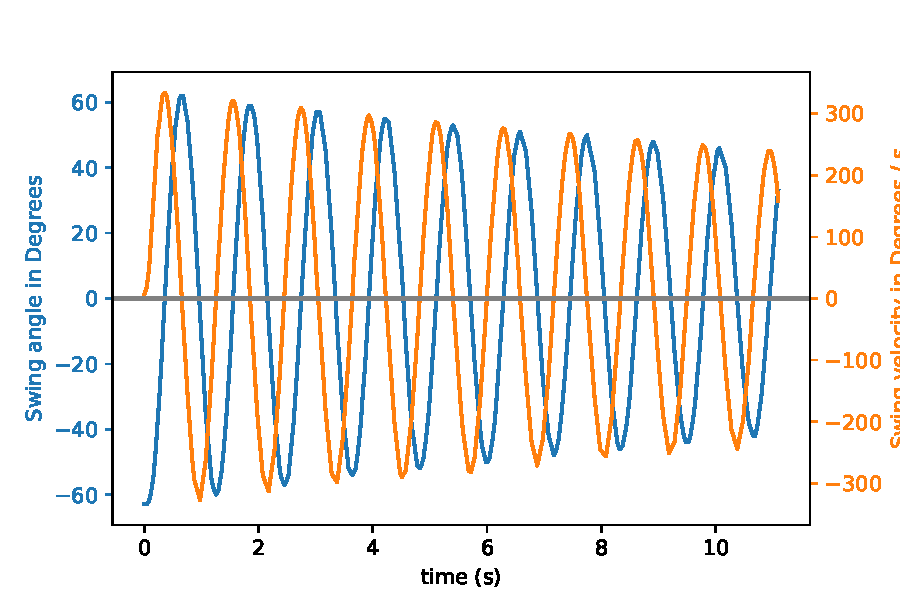
\includegraphics[width=0.6\linewidth]{images/pendulum}
		\caption{Measurement of a well calibrated gyroscope attached to a pendulum. Angle of the pendulum in blue, acceleration in orange. No drift in angle measurements is apparent in the 10 second timeframe.}
		\label{fig:pendulum}
	\end{figure}
	
	
	\pagebreak
	\section{Colour robot}
	We will now present the first of the three big robots that comprise the body of the project. We seek to have models that demonstrate and visualize machine learning and reinforcement learning at different levels of complexity. The first robot, presented here, represents the bottom level of complexity, and focuses on visualization of concepts rather than implementation of complex models.
	\subsection{Problem}
	A common first topic when learning about machine learning is the KNN algorithm, as it's simple to understand, allowing it to be a comparison for other models, or a base model to use when explaining other topics not specific to a model.
	
	The colour sensor was chosen as a way to visualize KNN. We wanted to be able to visualize how machine learning updated after data was added and what the basis for decisions were, using a simple and easy to understand setup, expanding on the simplicity of KNN by adding visual or even physical aids.
	\subsection{Robot Design}
	The robot was built to be easy to use and consistent to allow similar observations from the colour sensor at different times.
	
	A mount was made for the sensor, that easily plugged into the robot, and which could provide readings from everything placed on top of it, allowing for regular distances to the observed object at one regular LEGO Technic block. Two buttons where added to the side of the robot for controls.
	
	The final design is simple and modular, allowing it to be easily disassembled into smaller parts and reassembled later, and can be seen in Figure \ref{fig:colour_robot_full_shot}.\footnote{More pictures found in \texttt{additional\_robot\_images/Colour\_robot}.}
	
	\begin{figure}[H]
		\centering
		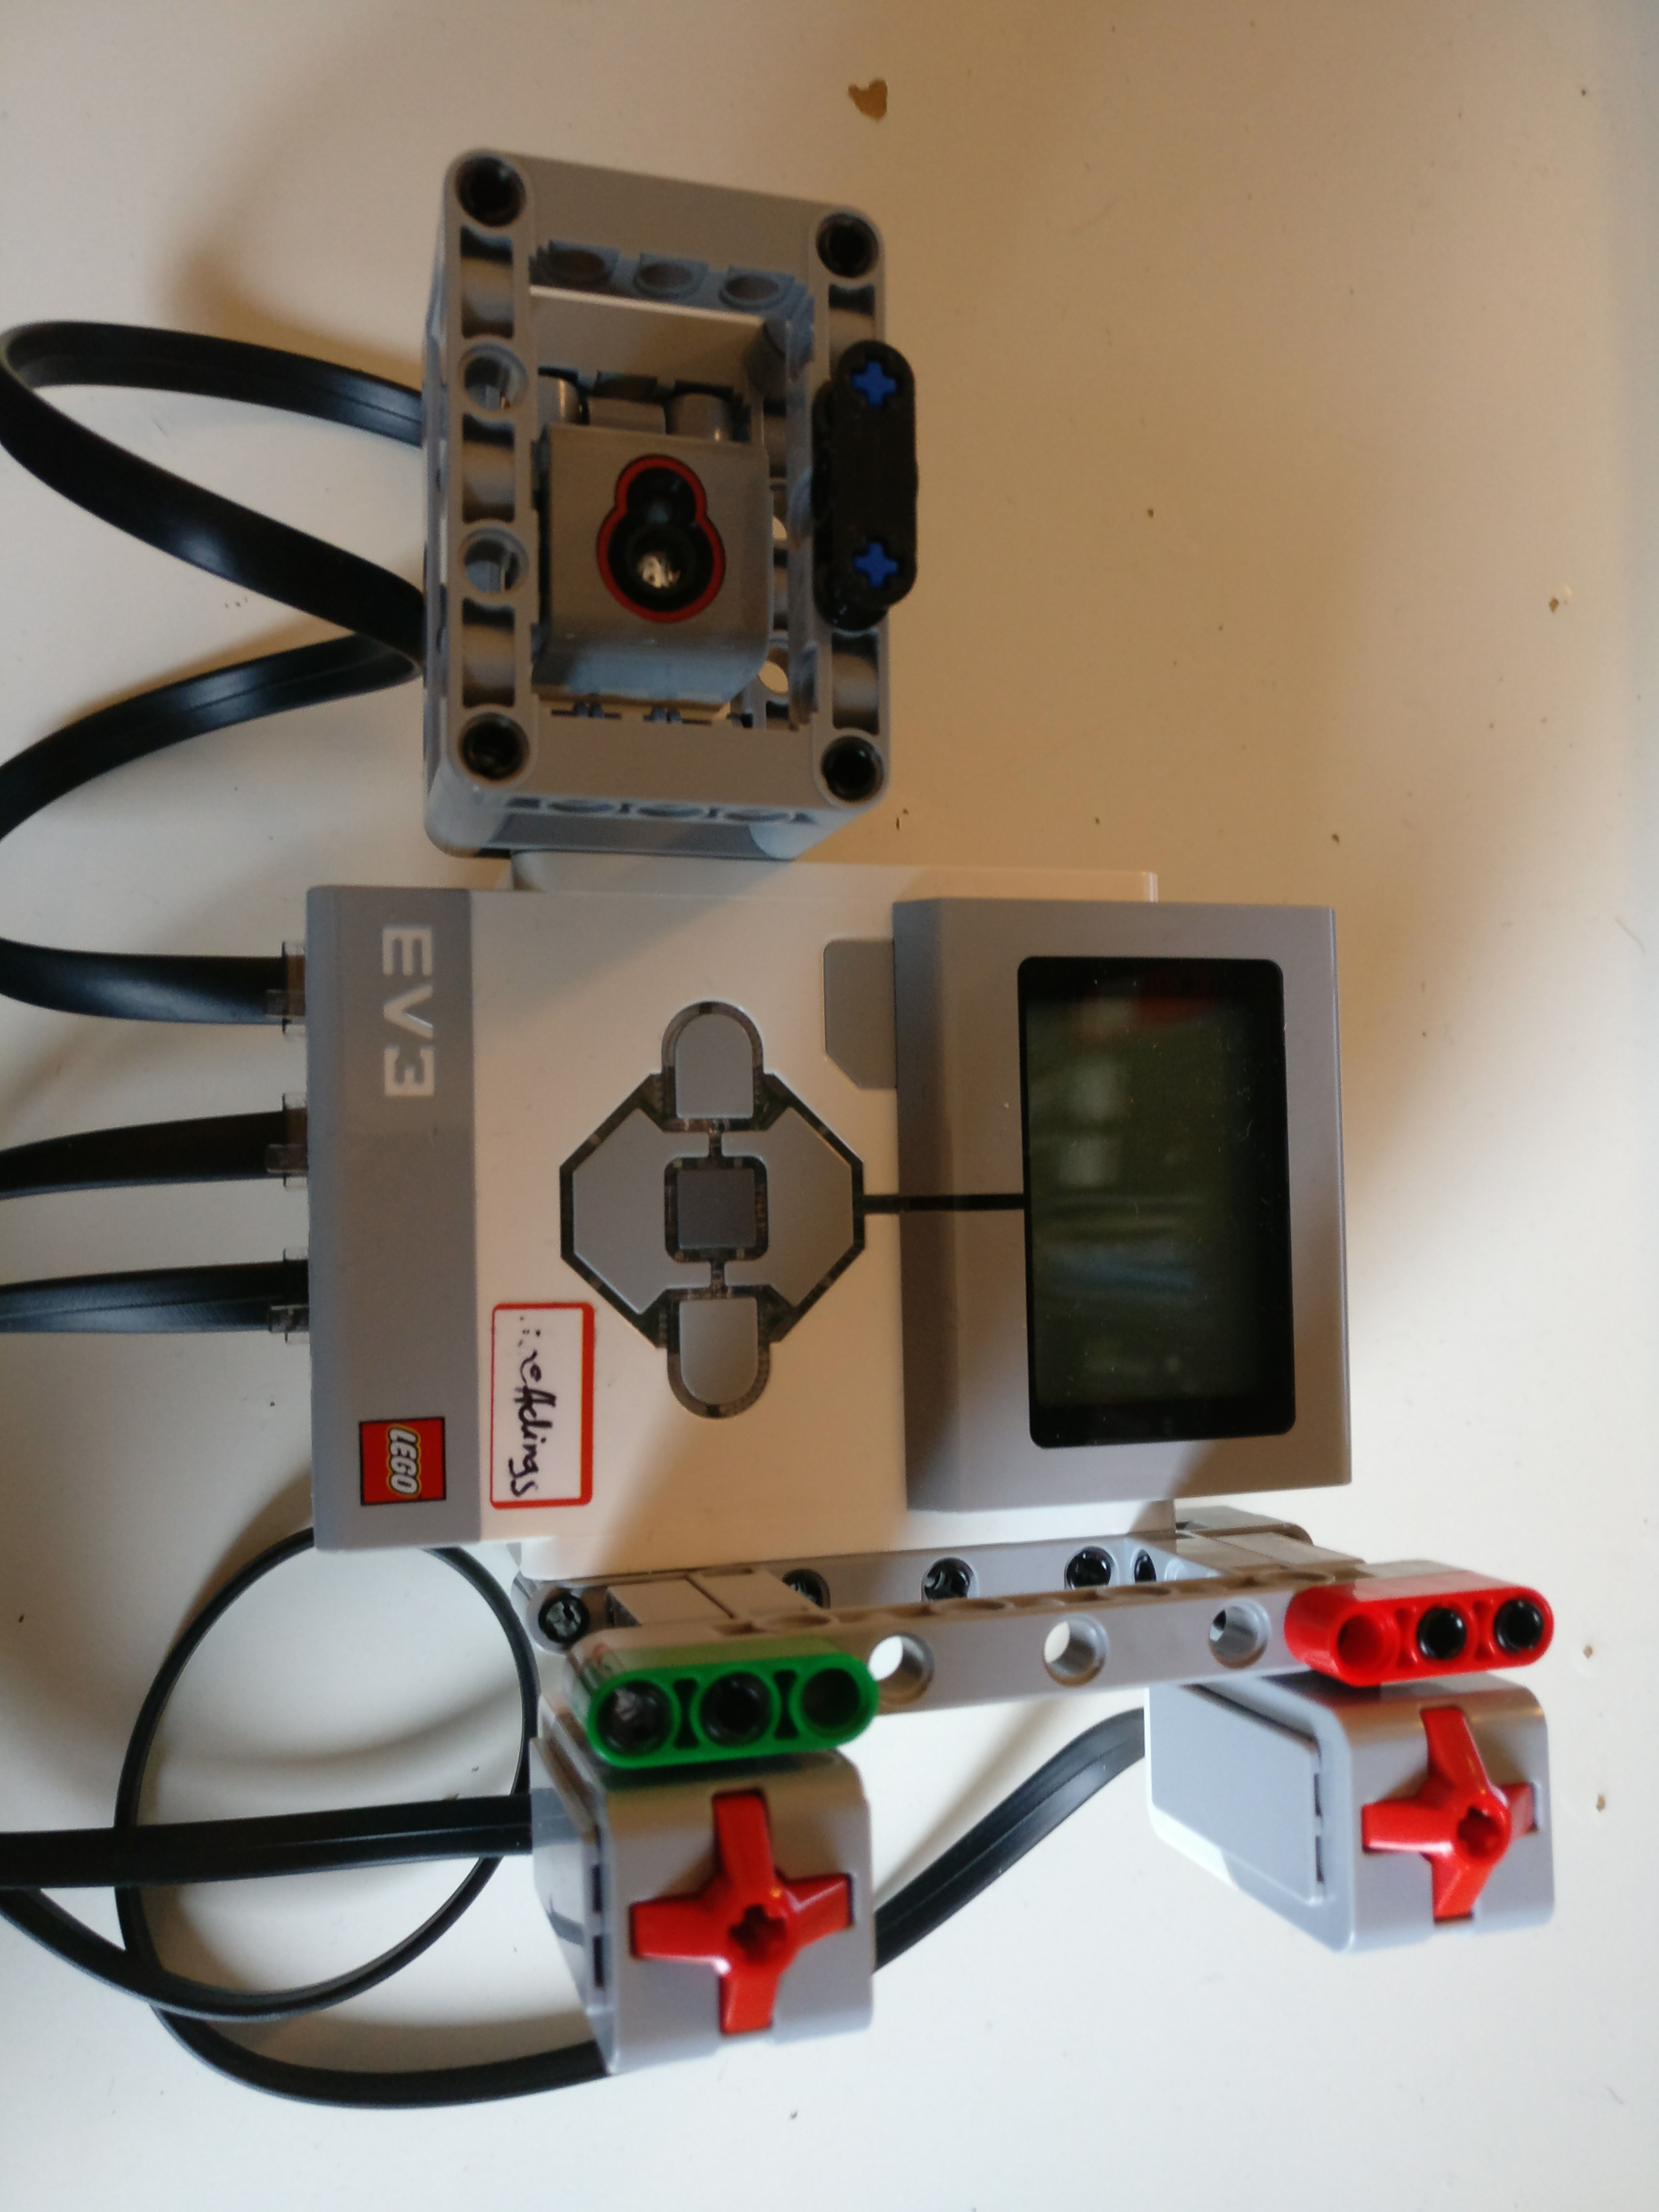
\includegraphics[angle=90,width=0.6\linewidth]{images/colour_robot_full.jpg} 	
		\caption{Full top shot of the colour robot, featuring the colour sensor and mount (left side), the brick (middle) and the buttons (right side).}
		\label{fig:colour_robot_full_shot}
	\end{figure}
	Since the robot has no moving parts, the results should be easily replicateable as along as the robot is built with two buttons and a color sensor, and the matter is kept still at a distance of one block.
	\subsection{The Learning}
	As planned we implemented KNN, as one of the simplest and most intuitive machine learning algorithms. For the data input we used only the RGB output from the color sensor. We wanted to plot in real time, and learned from the time-experiments that calling more values proved too much of a delay. For visualization, we used a 3D-plot of the observed colors, with the axes being red, green and blue values.
	
	We made two versions of KNN with the color sensor\footnote{The code for both of these is found commented in \text{simple\_learning/KNN colors.ipynb}.}, and a more advanced neural network model\footnote{The code for this is commented in \texttt{reinforcement\_colors/reinforced\_colors.ipynb}.}.
	\subsubsection{Colour learning: Internal LEGO based model}
	The first version is slightly silly, but colorful. Our dataset is started with either a base set (simple RGB values) or a few observations, in which we use the color sensor's built in predictions. Real-time KNN is then run, and we output our prediction as well as a 3D plot of our current observation (black triangle), together with all previous observations (coloured dots). Additional dots can be added by pressing a button, which adds the current observation and prediction as a true point in the data. This produces colourful plots, as seen in Figure \ref{fig:colour_KNN_LEGO}.
	
	\begin{figure}[H]
		\centering
		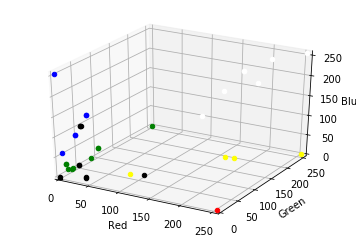
\includegraphics[width=0.6\linewidth]{images/ColourKNNversion1.png} 	
		\caption{Visualization output from the LEGO based KNN model. Here each coloured dot represents a data point with corresponding RGB values and the represented colour. Current observation, represented by a black triangle, is not featured.}
		\label{fig:colour_KNN_LEGO}
	\end{figure}
	\subsubsection{Colour learning: Binary classifier}
	Since the above version uses starting data and the built-in predictions from LEGO, we also tried a different setup. Instead of prediction colours directly, we predict colour groups, which we will call group "red" and group "green". In this setup, the robot again predicts and plots in real time, but we now start with zero data, and rely only on the buttons. One button adds the prediction to the data set with label "red" and the other "green". This allows us to not rely on anything from LEGO, and allows us to make different splits, such as light versus dark colours, which could learn to differentiate light and dark blue. The plots are similar to before, but with fewer colours, as seen in Figure \ref{fig:colour_KNN_binary}.
	
	\begin{figure}[H]
		\centering
		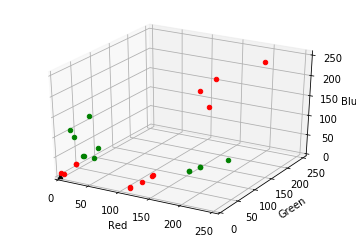
\includegraphics[width=0.6\linewidth]{images/ColourKNNversion2.png}	
		\caption{Visualization output from the binary KNN model. Here each coloured dot represents a data point with corresponding RGB values and the represented group. Current observation, represented by a black square, is seen in the bottom left, near (0,0,0).}
		\label{fig:colour_KNN_binary}
	\end{figure}
	\subsubsection{Colour learning: Neural Network and subject width}
	Finally, we implemented a more complicated system to work with other visualizations. We implemented a neural network, and wanted to visualize how learning and training works in this setup. 
	
	In this case, the robot has a list of allowed colors, starts with no data, and predicts from an untrained network. It reads RGB colours, but also reflected light and ambient light, since we are not running real-time. It displays scores for each color, and reads the highest scoring color aloud. A button press indicates whether this was correct or wrong, and it trains based on this feedback. This allows the user to view updates in predictions from step to step. The predictions are output on a list like below, updated with every new prediction
	\bigskip
	'Black : 0.13146167' \\
	\bigskip
	'Blue : 0.20897976' \\
	\bigskip
	'Green : 0.15094219' \\
	\bigskip
	'Red : 0.22930987' \\
	\bigskip
	'White : 0.14744666' \\
	\bigskip
	'Yellow : 0.13185982' 
	
	\subsection{Colour robot results}
	Two versions of a robot that uses KNN were implemented and built with visualization in mind. Both versions are functional, and can be used to explain and link how data affects predictions in machine learning.
	
	We implemented a simple Neural Network model, that may be useful in explaining more complicated machine learning models.
	
	We also learned a great deal about visualization and limitations to this, which will be presented and discussed in the following section.
	\subsection{Colour robot discussion}
	We encountered a number of difficulties related to these experiments, but have also found many avenues of possible future work.
	\subsubsection{Discussion: Visualization}
	We originally wanted to show the decision boundary for our learning system, to show how it changes with time. Unfortunately, we found no good way to visualize this in 3D, so instead we looked into dimensionality reduction. We tried reducing dimensionality using PCA, and plot a decision boundary in the resulting 2D space, but this proved problematic, both in our setup and generally. Since we wanted to run real-time we had issues running the PCA on the decision boundary. To get enough points for a proper boundary in 3D space we had to use at least 1 million points, which took way too long to process to be able to run real-time. If instead we didn't run real-time, we could plot the PCA values and a decision boundary in this space, but the values would be mostly meaningless. In the 3D space it at least somewhat makes sense, you have an intuition about what changes if we increase on the "red" axis and so on. In the PCA space we're left with principal components instead, and the points from previous observations would not even be stationary.
	
	Some ways to get around this issue would be to only read two colour channels (removing the need to reduce dimensionality), or find another experiment which only takes two inputs. 
	\subsubsection{Discussion: Neural Network and future work}
	The neural network setup was made to demonstrate that the colour sensor setup can be extended to more complicated machine learning systems, to show some width of the space of possible educational use. It was implemented, but as a very simple form. It takes a number of colours initially, and predicts between these, but for more than two colours (or colour groups) this makes training complicated. The model was implemented such that if it predicted the first colour on our list, and we respond correct, it trains with (1,0,0,0) (or similar for more colours) while instead if we respond wrong, it trains (0,1,1,1) (so it improves every other colour). 
	
	This setup is not optimal, and is simply a POC. If instead we want to focus on this task to improve it, it may be able to use methods from reinforcement or online learning, since we're dealing with a reduced feedback (right/wrong) setup (this was an idea from the start, as is obvious from the file name). The reason this wasn't implemented was a time constraint built into the setup. 
	\medskip
	
	At the moment, prediction is done by pressing both buttons, which causes the prediction list to update, and the robot to say the highest scoring colour. At this point you can press a button for yes or no. Unfortunately, you need a lot of observations to properly train the network, which makes it very time consuming and not very education-friendly. We ran a test with 150 entries, observing only Three different colours. After this, it could still not differentiate the Three colours. We believe that implementing a proper reinforcement or bandit setup would greatly improve the training, but 150 observations or just 50 that all have to be done manually is still a significant barrier for the neural network setup. 
	
	Other options could be to pre-load it with some amount of data, but this would remove the chance to see early learning. The output for the neural network model could of course be combined with a plot like the 3D we made for the KNN model, or a PCA/decision boundary or similar, with most of the same yields and issues as discussed before. We believe the neural network setup has potential, but has some hurdles to overcome before it can be useful in an educational setting.
	
	\pagebreak
	\section{Crawl robot}
	\begin{figure}[H]
		\centering
		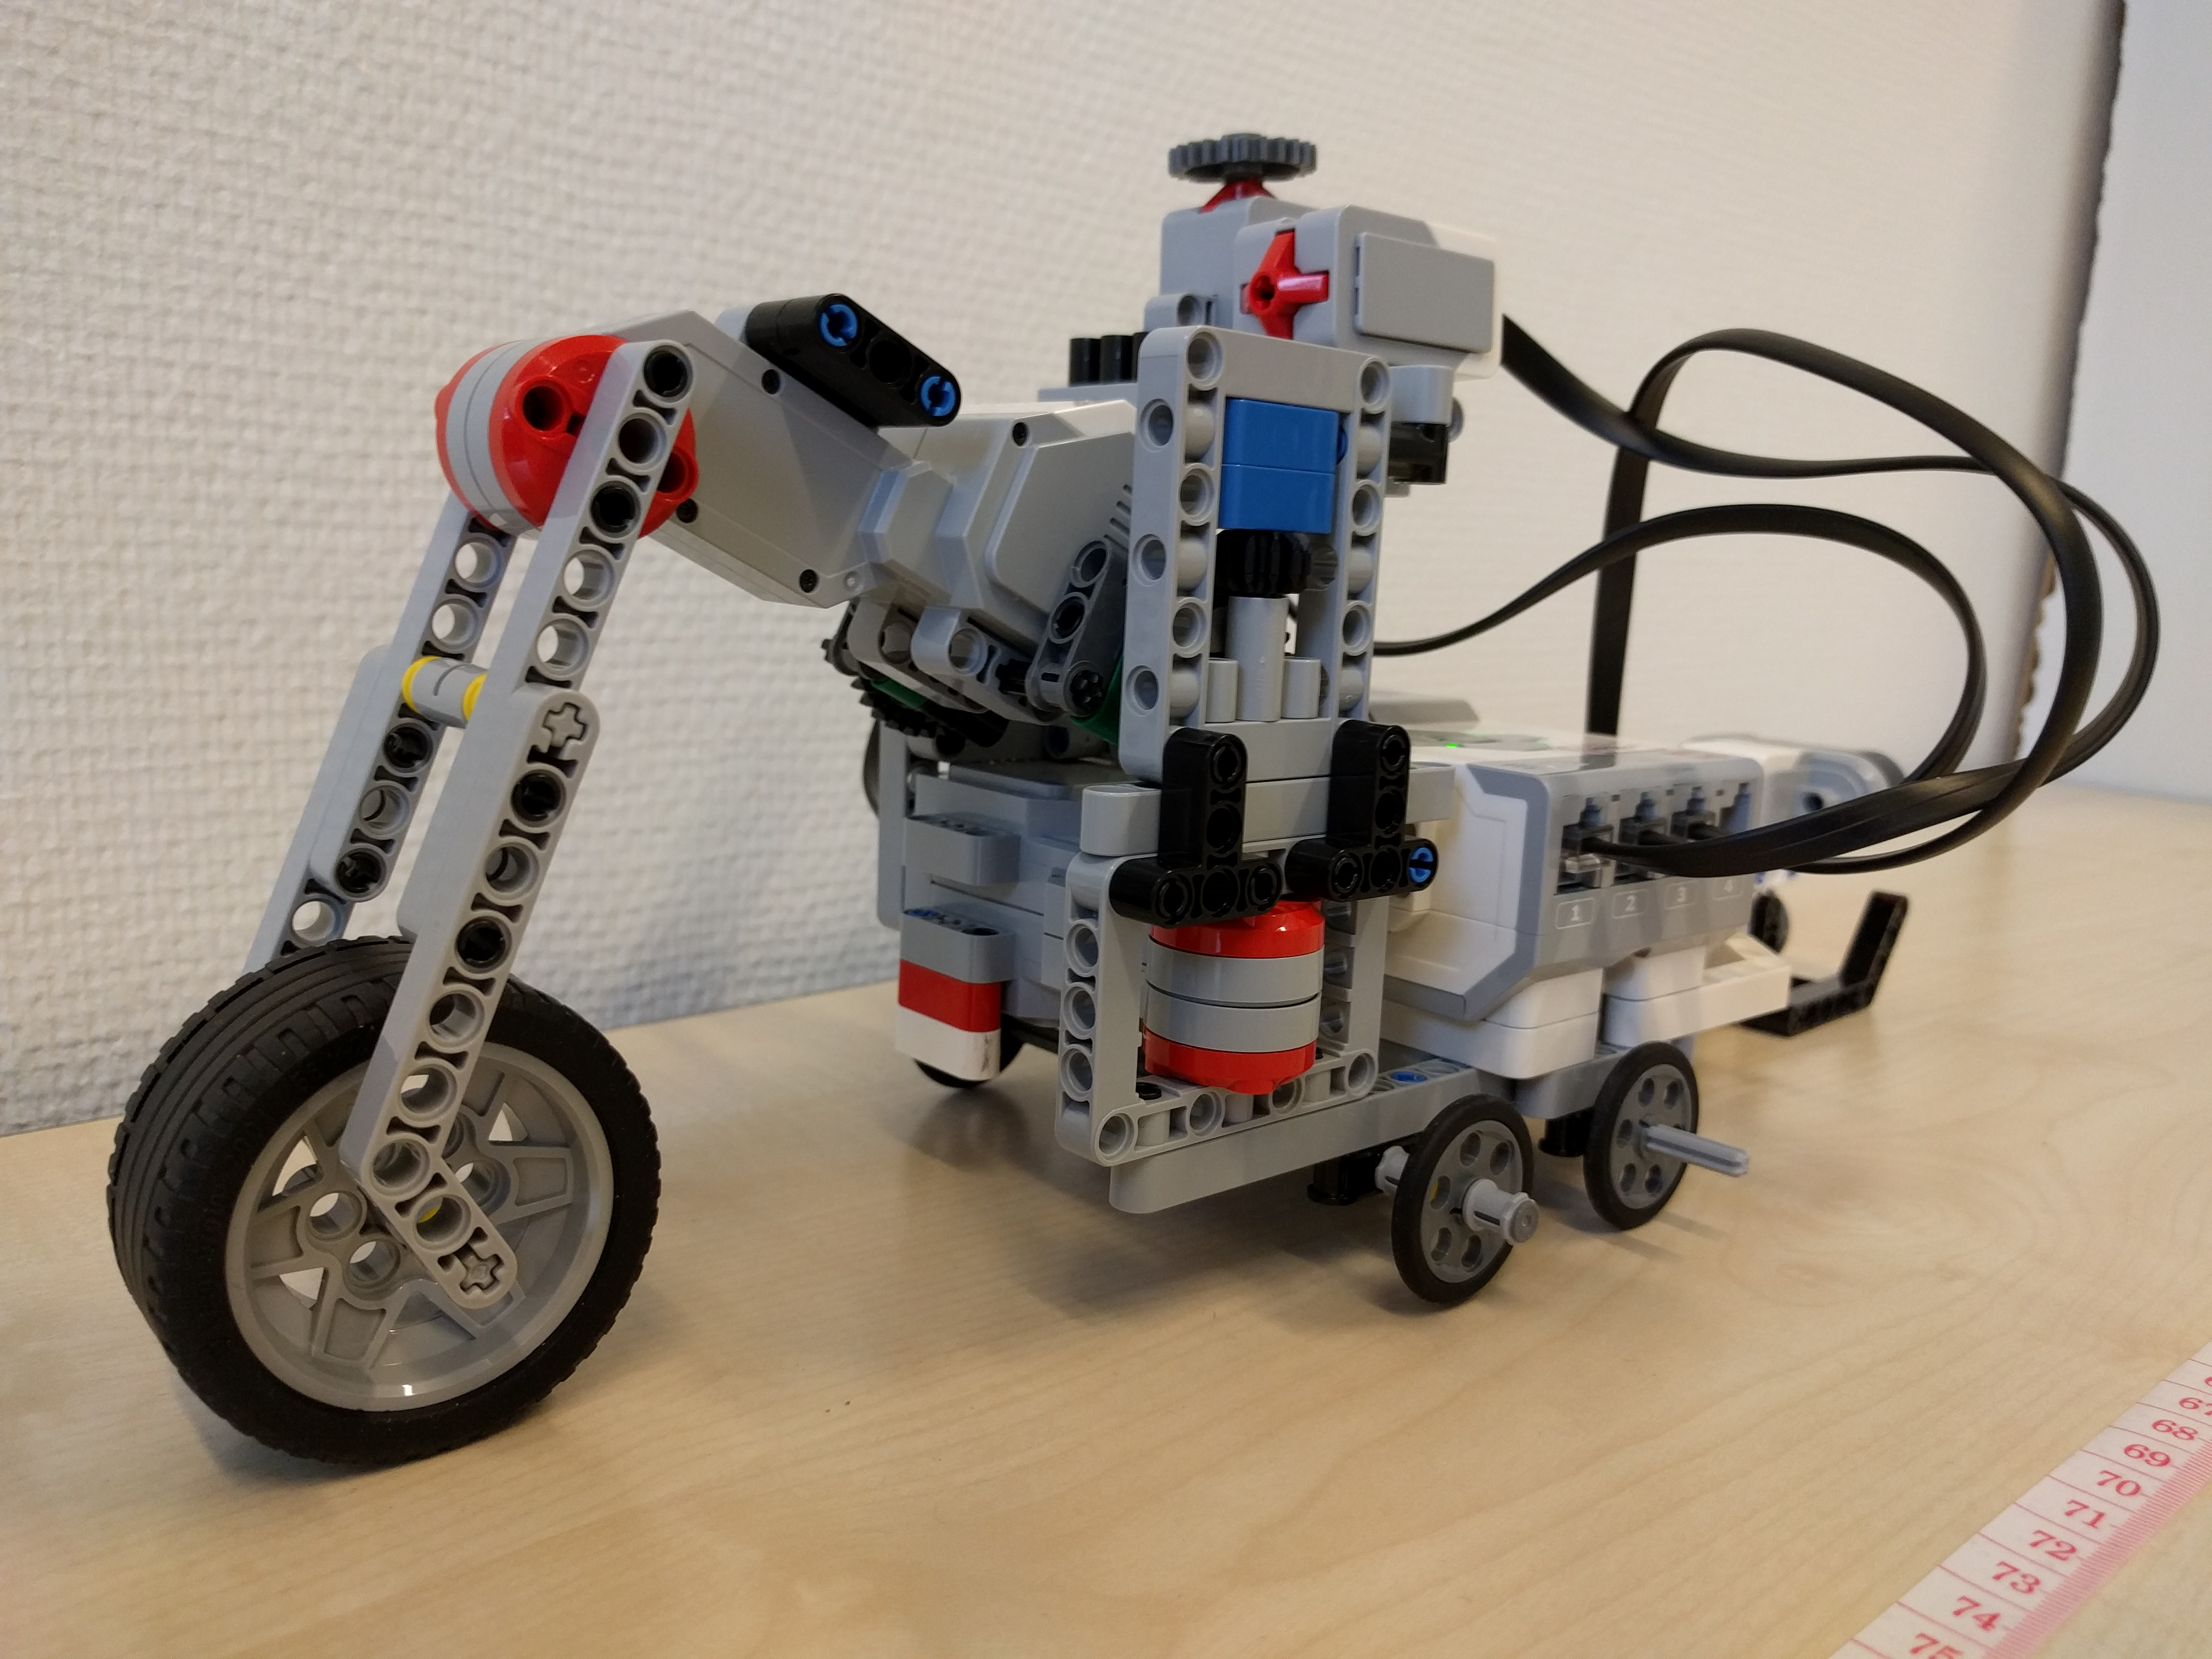
\includegraphics[width=0.6\linewidth]{images/crawl_robot}
		\caption{Crawl Robot, frontal view.}
		\label{fig:crawl_robot}
	\end{figure}
	To demonstrate reinforcement learning in educational settings, we seek to have a physical model for demonstration. The training process should be robust, as to deliver a reliable demonstration in teaching scenarios outside of laboratories, and fast, to keep the attention of an audience. While many robot designs and learning goals, like pole balancing or swinging, are possible, we selected a crawling robot as a suitable object for demonstration. The concept of a robot using one arm to crawl, or drag itself along a linear track has been explored by multiple other studies \cite{youtube_crawl2} \cite{youtube_crawl}. We selected this task, as it is a comparatively simple design, with few moving parts. The system is more robust towards external force from curious bystanders than for example a loosely swinging pole. By Defining a limited state space we can simplify the problem and get a training time suitable for demonstration. Realizing this robot will provide us with a model for demonstration  and equip us with the experience and knowledge to solve more complex problems in the future.
	
	
	\subsection{Robot Design}
	To facilitate the crawling motion, the robot needs a movable arm to pull itself forward. The arm consist of two elements; the base arm, which is attached to the robot, and a pivot arm attached to the base arm. Both arm joints rotate around the same axis, allowing the hand at the far end of the pivot to move on a plane. To allow the arm to pull the robot, the ground friction of the arm has to be maximized, and the ground friction of the robot minimized. This is achieved by a big rubber tyre firmly attached (not spinning) to the robots hand. The robot body sits on wheels which can spin freely. See Figure \ref{fig:crawl_robot} for a photo of the robot arm, hand and wheel basis.
	
	To measure distance travelled, the ultrasonic sensor is used. This sensor is attached to the back of the robot and records the distance to a target from the rear end of the robot. As the wheel basis of the robot might tilt when the arm is pressing into the ground, while the ultrasonic sensor requires a stable angle towards the target for consistent measurements, the sensor is mounted on a sled which is pulled behind the robot. The sled is visible in Figure \ref{fig:sub2}.
	
	To calibrate the motors of the arm, two buttons are attached to the top of the robot. During the start up process, the arm is moved all the way back, until base arm and pivot arm hit their respective buttons. This motion is depicted in Figure \ref{fig:sub1}. The certainty about the arm position attained by this action is used to initialize the zero-angle of both motors.
	
	\begin{figure}[H]
		\centering
		
		\begin{subfigure}{0.4\textwidth}
			\centering
			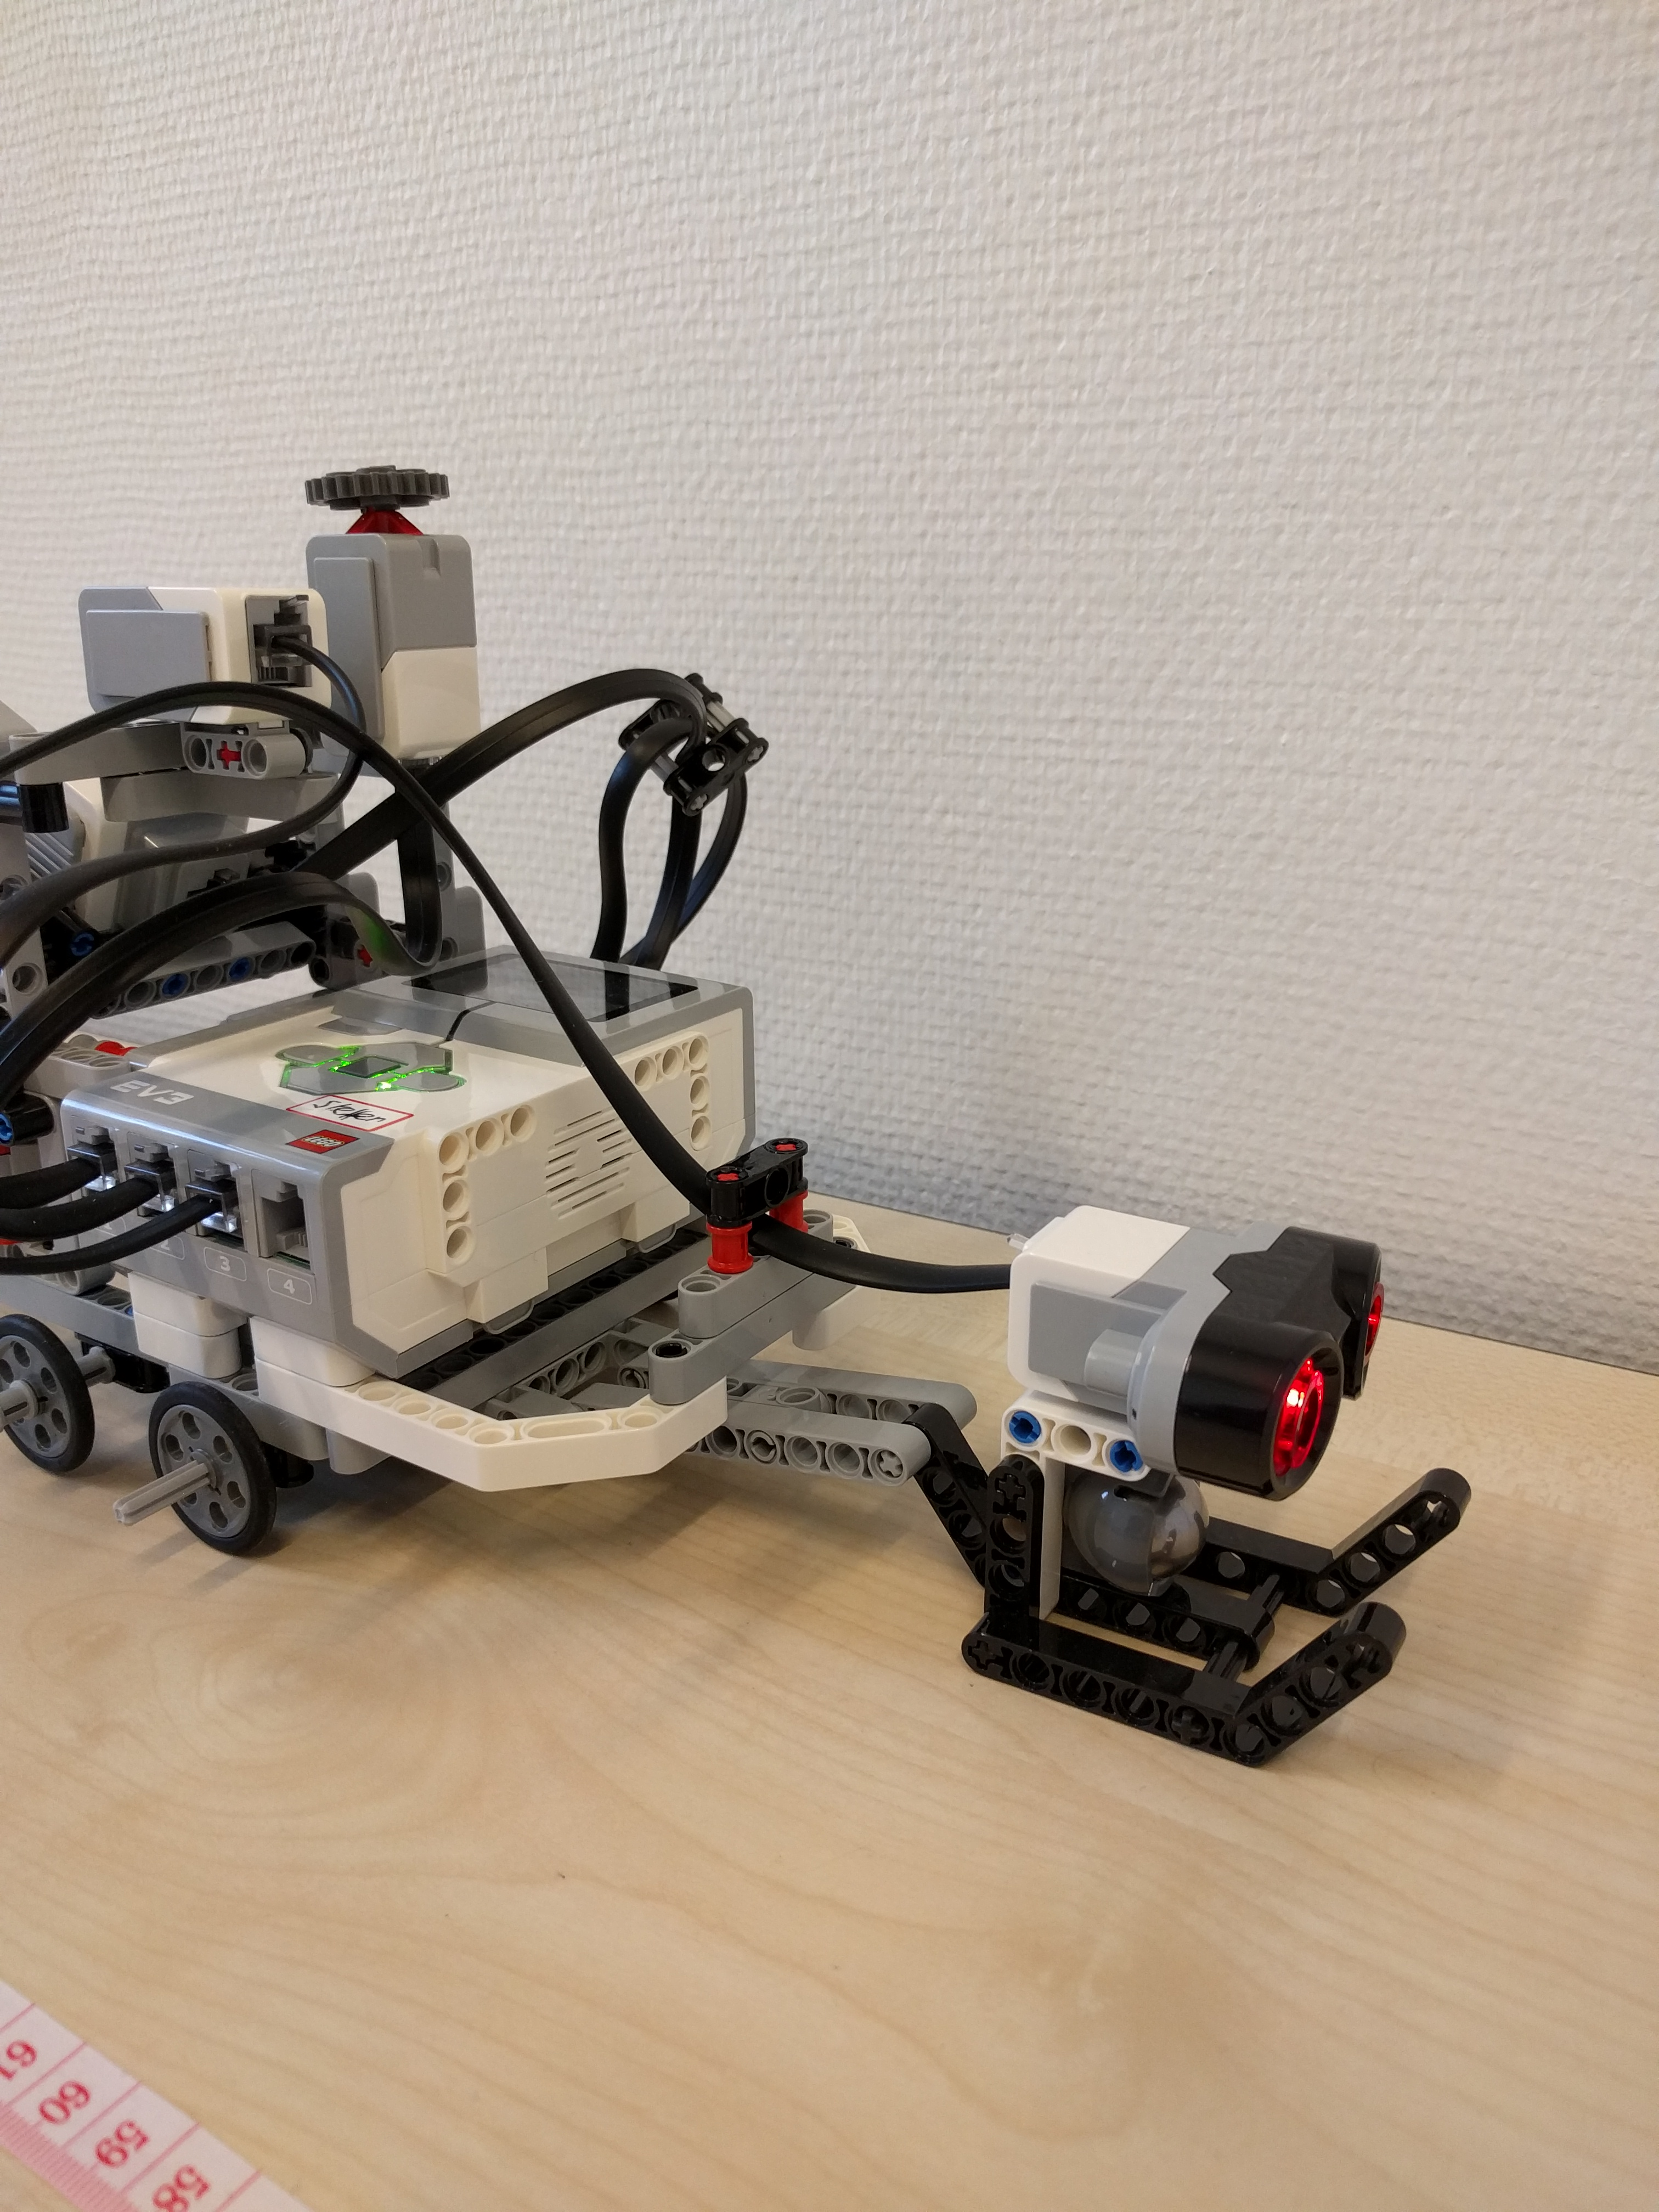
\includegraphics[width=0.8\linewidth]{images/crawl_sled}
			\caption{Ultrasonic sensor on a sled at the back of the robot.}
			\label{fig:sub2}
		\end{subfigure}
		\begin{subfigure}{.4\textwidth}
			\centering
			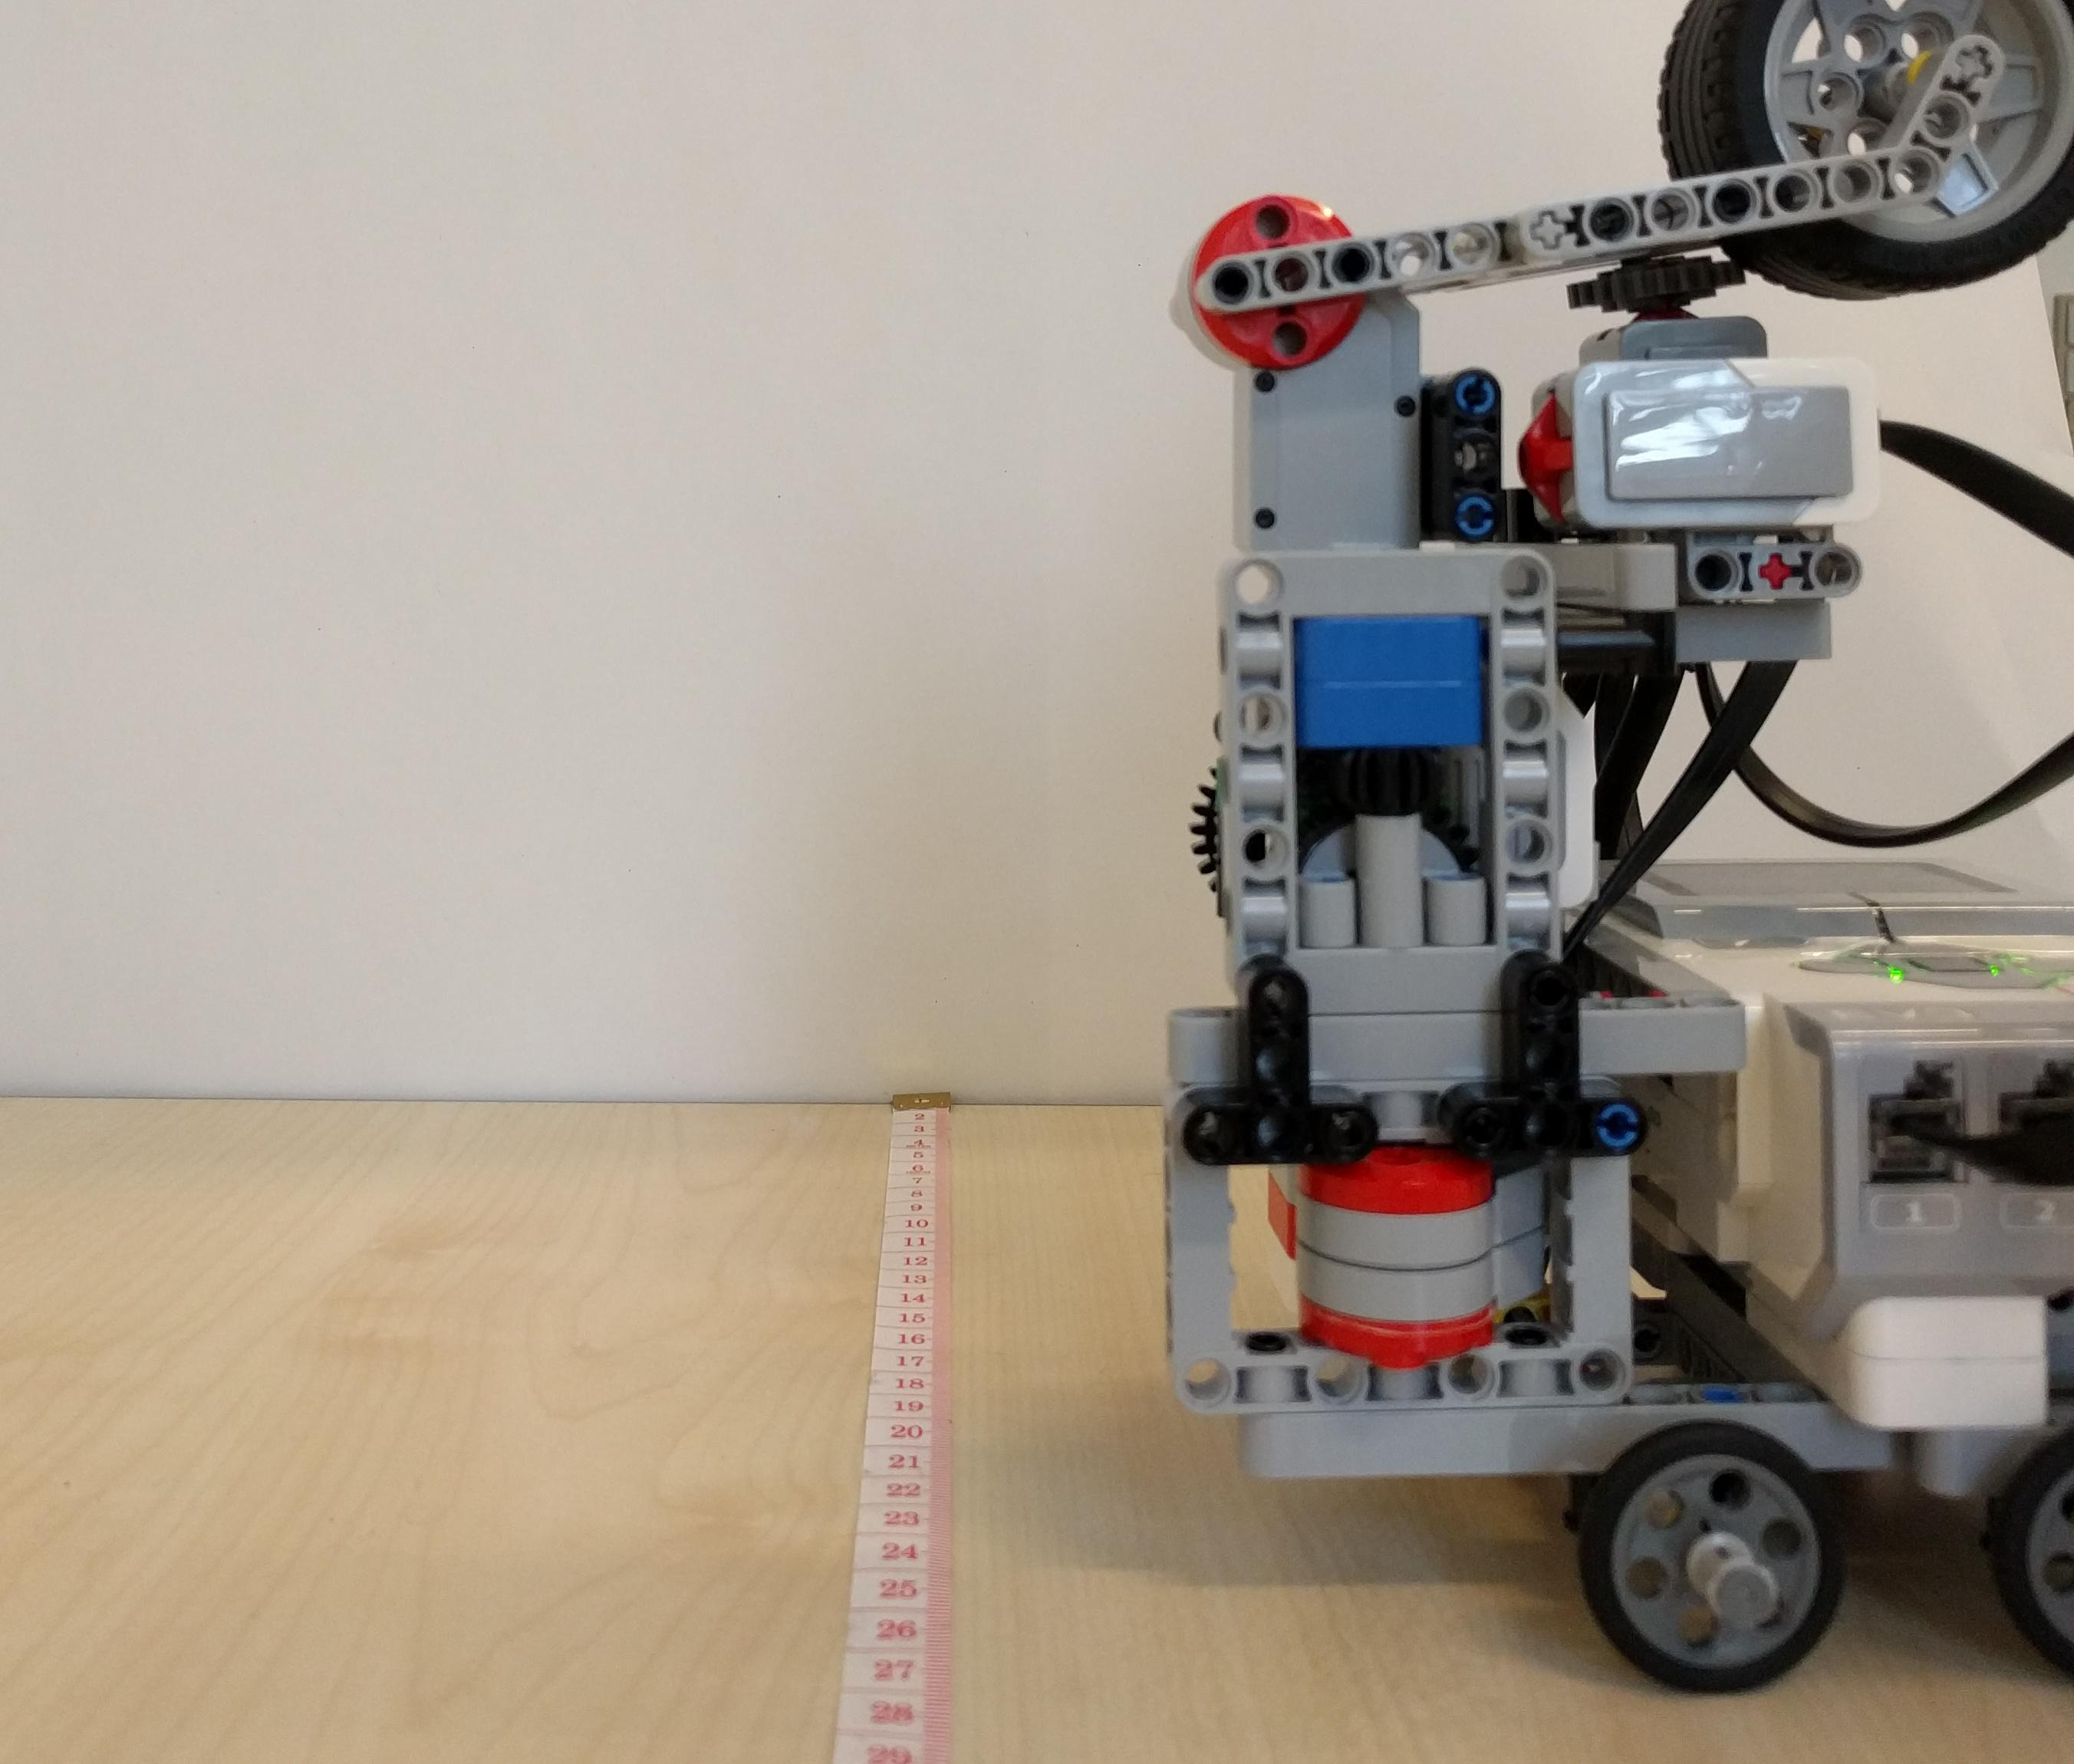
\includegraphics[width=1\linewidth]{images/crawl_calibrate}
			\caption{Calibrating motion of the crawl robot.}
			\label{fig:sub1}
		\end{subfigure}%
		\caption{Designs of the Crawl Robot}
		\label{fig:test}
	\end{figure}
	
	\subsection{Formulation of the Learning Problem}
	To train the robot how to crawl, we use Q-learning. Q-learning is a form of reinforcement learning. It provides agents with the capability of learning to act optimally in Markovian domains by experiencing the consequences of actions. To learn, an agent tries an action at a particular state, and evaluates its consequences in terms of the immediate reward or penalty it receives and its estimate of the value of the state to which it is taken. By trying all actions $A$ in all states $S$ repeatedly, it models the value $Q(s,a)$ of each action state pair. The algorithm learns which state-actions pairs are the best overall, judged by long-term discounted reward \cite{Watkins1992}.
	
	\begin{figure}
		\centering
		\includegraphics[width=0.6\linewidth]{images/crawl_states}
		\caption{Arm positions (states) of the crawl robot. From top to bottom: Pivot arm in positions far, mid, close. From left to right: Base arm in positions up, mid, down. The tilt of the robot base in the right column is caused by the arm pressing into the floor.}
		\label{fig:crawl_states}
	\end{figure}
	\medskip
	The Q-learning algorithm fits the domain of the crawl robot. The implementation chosen is shown in Algorithm \ref{alg:q-learn} and follows \cite{sutton1998introduction}. Training is grouped into epochs, and each epoch consists of multiple steps (loops in line two and four of the algorithm). In each step, we take one action. This action is determined with the $\epsilon$-greedy strategy (lines 5-10), where with probability $\epsilon$ we perform a random action, and with probability $1-\epsilon$ we greedily select the action $a$ with the highest current value. In line 11 we perform the sampled action $a$, observe the reward $r$ and transition into the next state $s'$. In line 12 the state value function $Q(s,a)$ is updated. We end the step by setting $s \leftarrow s'$ and then repeating (line 13, 14). Each epoch starts with start state $s_0$. To execute the learned policy, we set $\epsilon$ to $0$ and no longer update the state value function.
	\medskip
	
	To apply Q-learning to the crawl robot domain, we model an action as moving the arm. The immediate reward or penalty received is proportional to the distance traveled by performing the action, as measured by the ultrasonic sensor. As learning speed is of importance, we define a discrete state space with nine states. These states are displayed in Figure \ref{fig:crawl_states}. By selectiong the state space to be small, the learning algorithm has to explore only few states, which speeds up learning. We could have sub divided the arm movement plane into more states, with the drawback of longer learning time. More formally, the choices for the action-space $A$ and state space $S$ are:
	\begin{align*}
	A = \{ &\text{ move base arm up}, \text{ move base arm down} , \text{ move pivot arm far}, \text{ move pivot arm closer}\} \\
	S = \{ &\text{base up pivot far}, \text{ base mid pivot far}, \text{ base down pivot far}, \\
	&\text{base up pivot mid}, \text{ base mid pivot mid}, \text{ base down pivot mid},\\
	&\text{base up pivot down}, \text{ base mid pivot down}, \text{ base down pivot down},\} \\
	\end{align*}
	The initial state for each epoch is given by $s_0 = \text{base up pivot far}$, which is the furthest extension of the arm. For fast learning, we got good results with a learning rate $\alpha = 0.5$, discount rate $\gamma = 0.8$. The exploration factor $\epsilon$ is initially set to $0.5$ and declines exponentially throughout training, allowing lots of exploration at the start of training, while gradually reducing exploration for later epochs. We chose $35$ steps per epoch, as this amount allows each epoch to explore all states multiple times. Training is stopped once the motion appears to be executed with little error.
	
	\begin{algorithm}[H]
		\SetKwInOut{Input}{Input}
		\SetKwInOut{Output}{Output}
		
		\Input{learning rate $\alpha \in ]0,1]$, discount rate $\gamma \in [0,1[$}
		initialize $Q(s, a)$ with $0$ for all $s,a$\\
		\ForEach{epoch}
		{
			return to initial state $s_0$ \\
			\Repeat{epoch end}
			{
				sample $x$ uniform at random for $[0,1]$ \\
				\eIf{$x < \epsilon$}
				{sample $a$ at random}
				{select $a \leftarrow \arg \max_a(Q(s,a))$}	
				take action $a$, observe $r, s'$ \\
				$Q(s,a) \leftarrow Q(s,a) + \alpha [r + \gamma \  max_{a'} Q(s', a') - Q(s,a)]$ \\
				$s \leftarrow s'$
			}
			
		}
		\Output{state value function $Q$}
		\caption{Q-learning with $\epsilon$-greedy exploration}
		\label{alg:q-learn}
	\end{algorithm}
	
	
	
	
	
	\subsection{Crawl robot results}
	The crawl robot was trained using tabular Q-learning with the parameter choices stated in the previous section. In this section we present the training process and the learned result. For training, the robot is placed on a linear track. At the back of the robot, a solid target is placed to act as a point for range measurement by the ultrasonic sensor. During training, the robot explores actions and moves back and forth on the linear track. 
	
	After 20 minutes of training, the learned motion appeared near perfect and training was stopped. This corresponds to 65 epochs of training, for a total of 2275 actions. The reward gathered in each epoch is plotted in Figure \ref{fig:crawl_reward}. We can see that the reward gathered in each epoch has a clear upward trend, indicating that the robot got progressively better at the task. The exploration factor is exponentially declining, as shown in Figure \ref{fig:crawl_exploration}. This leads to less exploration in later epochs. The result of this is visible in the reward plot, as in later epochs the results get more consistent.
	
	The robot is not fully autonomous during training. It requires human intervention in three cases:
	\begin{itemize}
		\item The ultrasonic sensor has a maximum range of 250cm. If the robot moves further away from its range measuring target, it can no longer track rewards. Similarly, if it pushes into the range finding target, it can not move further into the direction of the target. Both cases disrupt assessing the rewards of actions. To handle these cases, the robot will interrupt training when it gets too close to either end of the spectrum. Training is resumed once the robot is manually placed on a valid part of the training track.
		\item To properly assess the range to it's range measuring target, the ultrasonic sensor needs to be orthogonal to the target. If the robot rotates during training, the angle to the range finding target can change. An angle significantly different from 90 degrees leads to skewed reward tracking, and in special cases the sensor can no longer find the target, which prohibits range measuring entirely. If the orientation of the robot changes significantly, it has to be manually rotated to its initial position.
		\item In rare cases, the motors of the arm have slightly too little torque to push against resistance caused by the hand hitting the floor. The motors become stuck. In these cases the robot needs to be slightly pushed to overcome the resistance and release the motors.
	\end{itemize}
	
	A recording of the full training and a presentation of the learned motion is accessible as a video online\footnote{Available at \url{https://youtu.be/NUTv-oNWEYo}.}. The video shows the training process at seven times normal speed. Manual interaction is shown as well.
	
	\begin{figure}[H]
		\centering
		\begin{subfigure}{.48\textwidth}
			\centering
			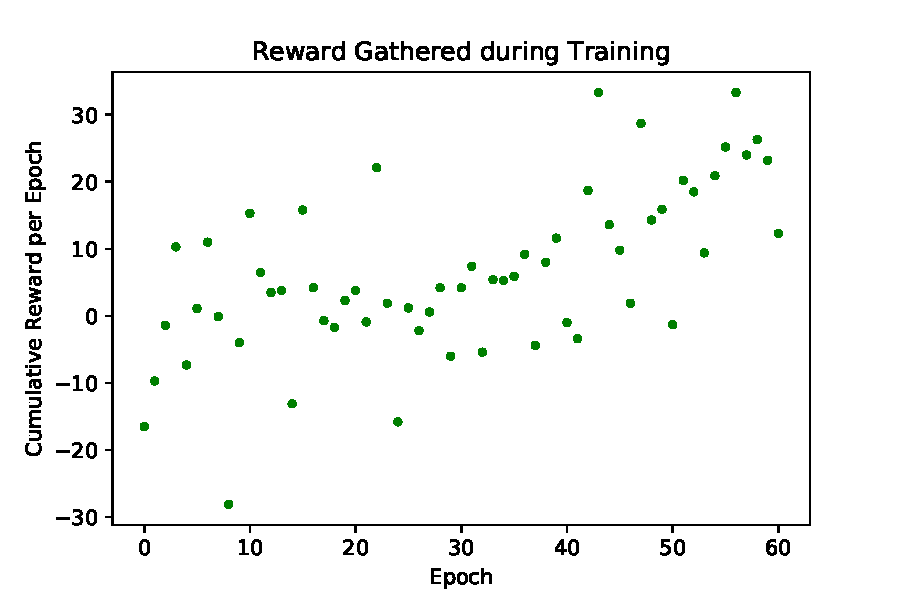
\includegraphics[width=1\linewidth]{images/crawl_rewards}
			\caption{Reward gathered per Epoch. An improvement is clearly visible.}
			\label{fig:crawl_reward}
		\end{subfigure}
		\begin{subfigure}{.48\textwidth}
			\centering
			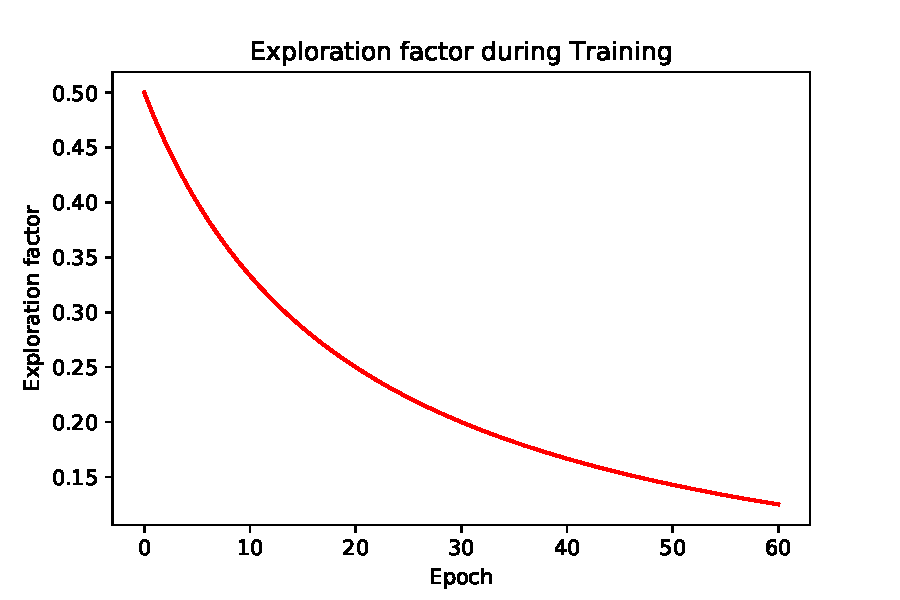
\includegraphics[width=1\linewidth]{images/crawl_exploration}
			\caption{Exponential decline of the exploration rate.}
			\label{fig:crawl_exploration}
		\end{subfigure}%
		\caption{Q-learning of the Crawl Robot}
		\label{fig:crawl_train}
	\end{figure}
	
	
	\subsection{Crawl robot discussion}
	With the presented framework, the crawling robot is able to learn a forward crawling motion in 20 minutes. As the training process requires constant human interaction for resetting the robot, we think this amount training time is appropriate. Especially in educational settings it should be considered as an upper limit. Since the training is interactive, observing how the robot develops an increasingly stronger forwards drive during training is quite rewarding to the observer. 
	
	The learned motion is not smooth and appears abrupt, which results from the use of a discrete state space. Learning a crawling motion with this robot on a continuous state space has the potential of leading to a smoother, and possibly faster movement. A possible drawback is increased training time. Moving the arm on a continuous state space is a topic for future research.
	
	The robot construction can be improved in the future. The current design has some mechanical issues, such as the strength of the motors in the arm and a tendency to slightly drift off the linear direction of movement. These problems could be addressed by re-constructing the robot and track of movement. A guide rail could constrict sideways the movement and gear conversions in the arm can be used to increase torque. The need for human supervision could be reduced by introducing a third motor to automatically move the robot back to its starting position after every epoch.
	
	\medskip
	In conclusion, we build a one-armed robot using LEGO parts, motors and sensors. We formulated a tabular q-learning problem with the goal of teaching the robot how to crawl. With some human interaction, the robot learned a forward crawling motion in 20 minutes.
	
	
	
	
	\pagebreak
	\section{Swing-Robot}
	With the colour detection and crawling robots we demonstrated two robots that can be used in an educational environment to experience interactively how machines learn and improve. We now focus on a bigger, more imposing robot that can be used as an exhibition piece to demonstrate what machine learning is capable of achieving. The swing-robot is a robot attached to a freely swinging pendulum. The robot tries to swing the pendulum back and forth by its own movements. The goal is to learn a sustained, rapid swinging motion. 
	
	We select this more challenging problem, inspired by a similar robot found on YouTube \cite{youtube_swing}. In this setup, the robot has to learn to swing, by swinging one or both legs back and forth, and will receive higher rewards the higher it swings. This creates several layers of complexity. The task is time sensitive, as the swing moves freely, and we need to be able to react fast to the current motion. Observing the state of the system is significantly harder here, as measurements are constantly changing. The choice of the reward function is not obvious either.
	
	
	\subsection{The Robot}
	The two basic robot designs seen in the video that inspired this idea \cite{youtube_swing} can be described as a "crouch"-style swing, in which the robot does up-down body movements, and a "pull-up"-style swing, in which the robot moves legs/limbs to swing.
	
	We decided to build a "pull-up" style swing, where the corpus of a humanoid shaped robot is fixed to a harness, and only the robots legs can move. See Figure \ref{fig:swing_robot} for the construction of our robot.
	
	\begin{figure}[H]
		\centering
		\begin{subfigure}{.48\textwidth}
			\centering
			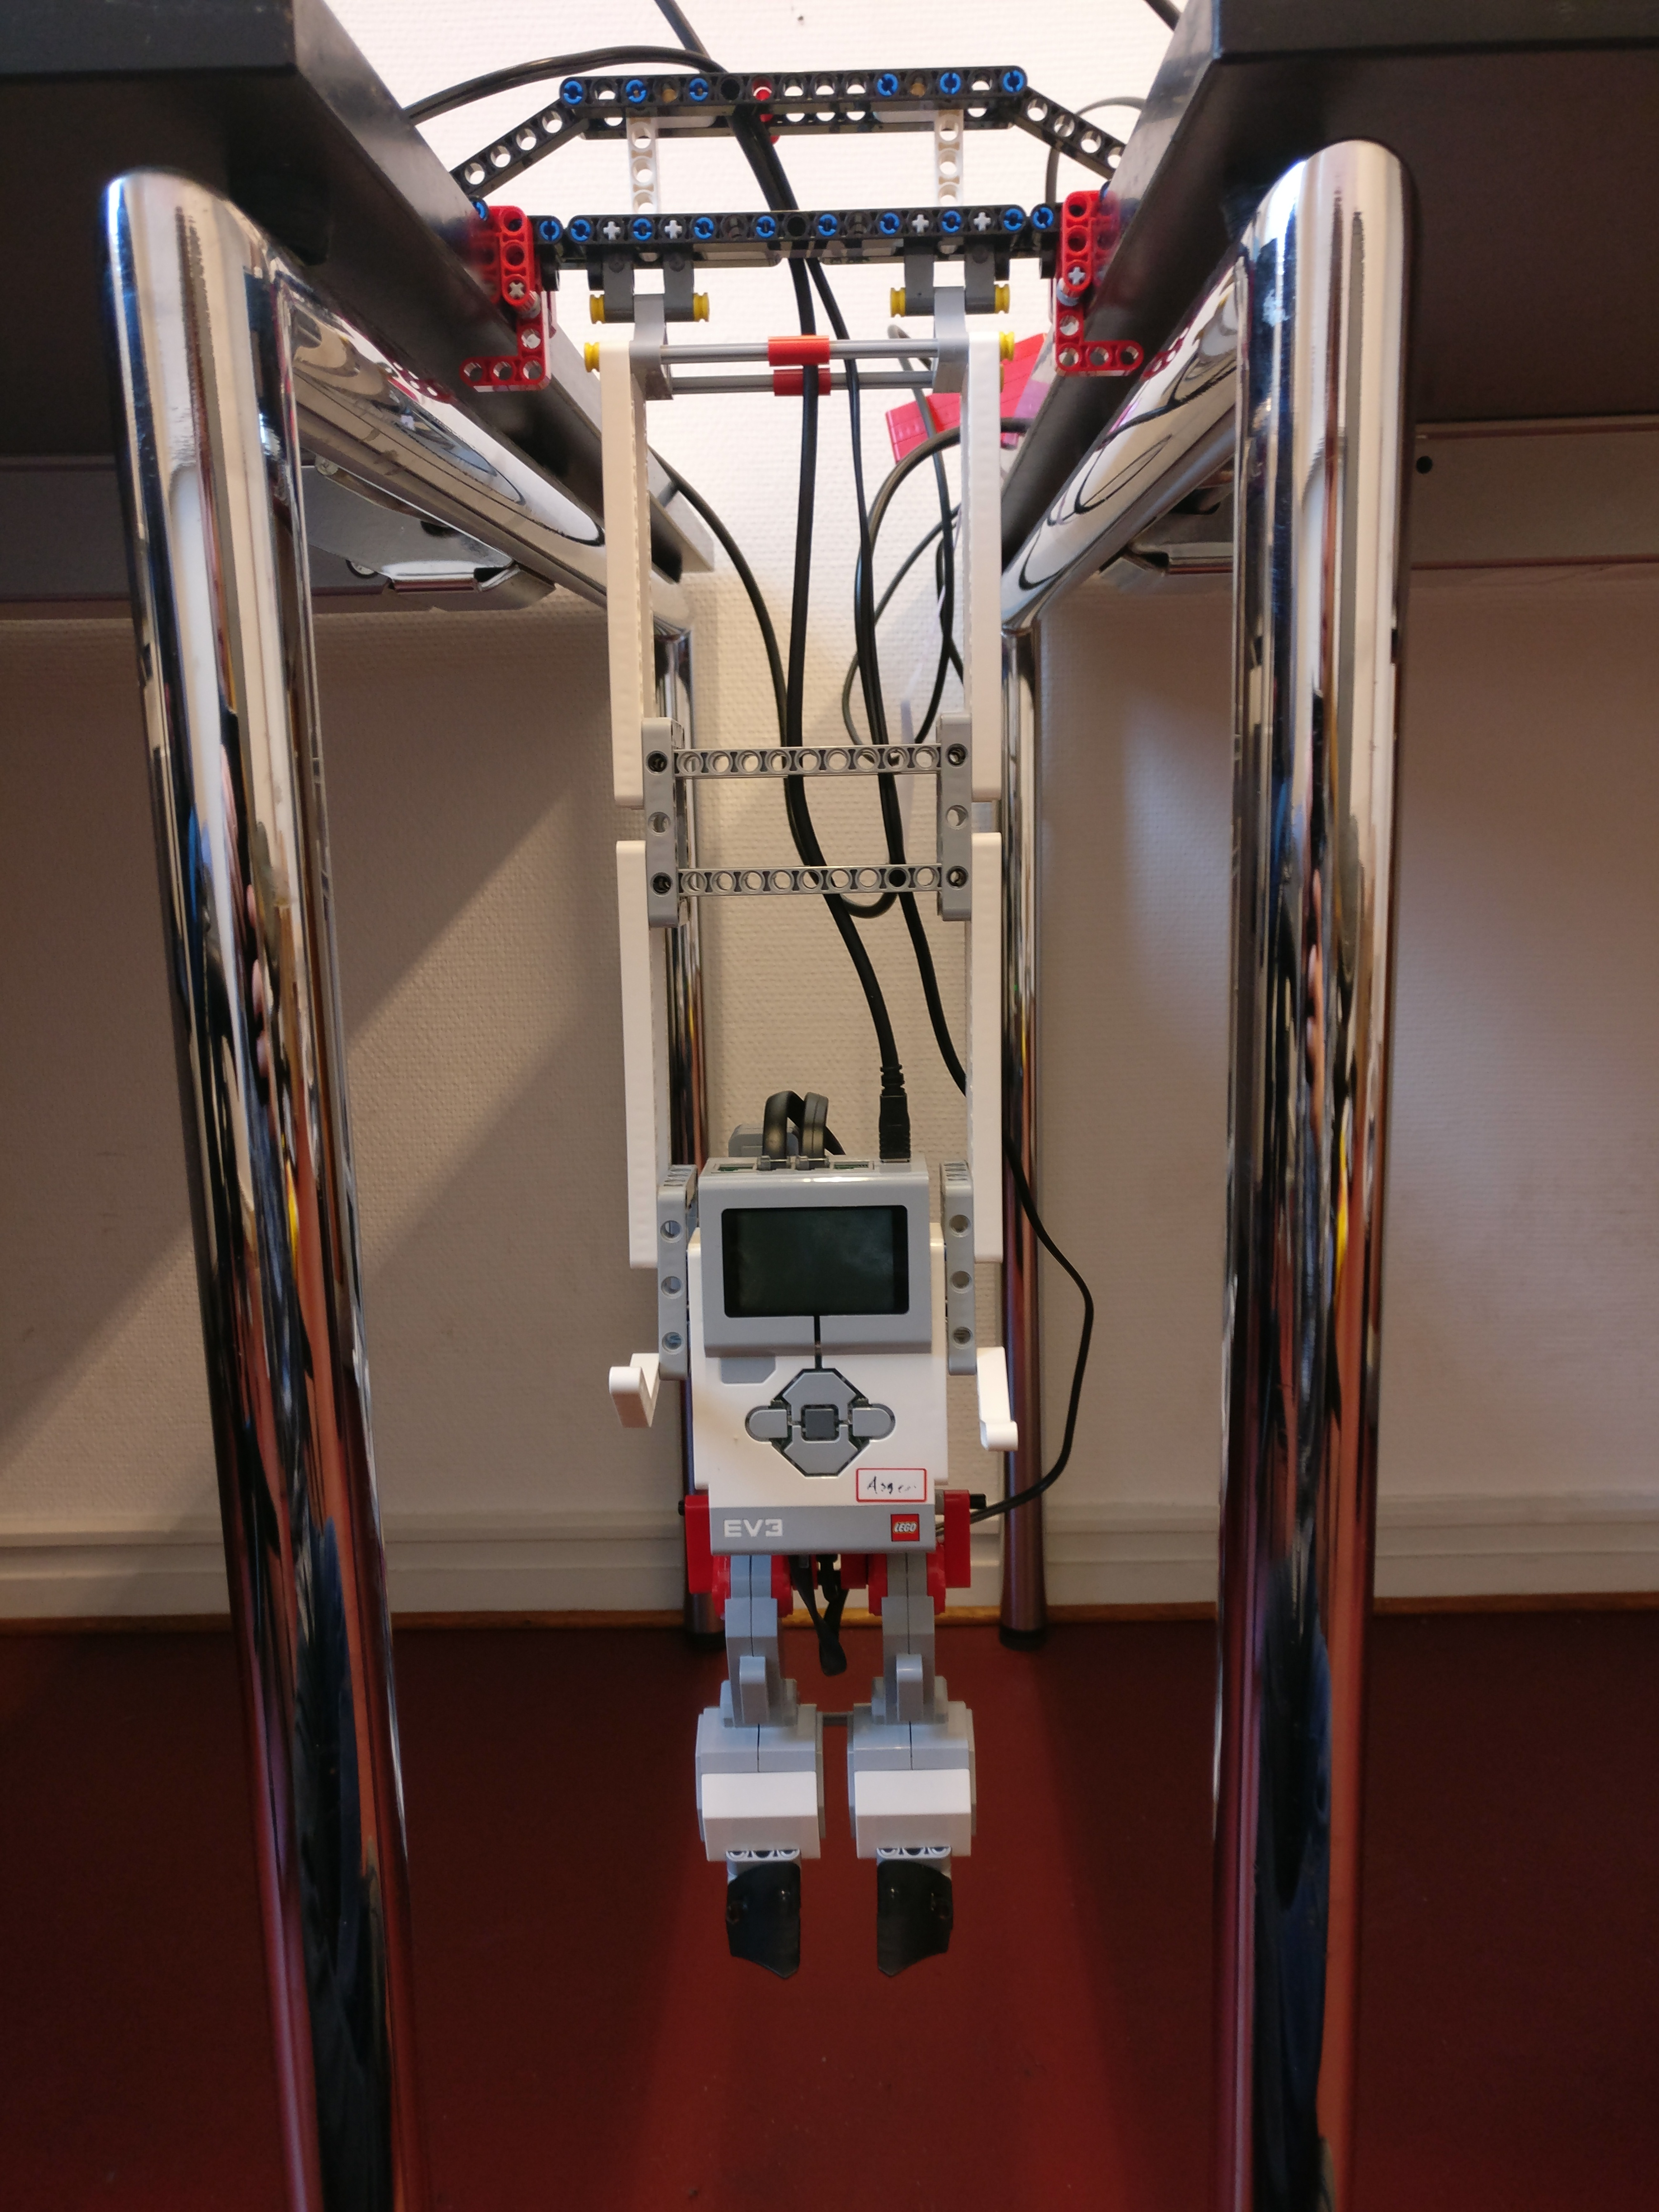
\includegraphics[width=1\linewidth]{images/swing_robot_front_full}
			\caption{Swing robot, frontal view. At the top of the picture you can see the robot mount lodged between two tables, the structure in the middle is the harness.}
			\label{fig:swing_robot_front}
		\end{subfigure}
		\begin{subfigure}{.48\textwidth}
			\centering
			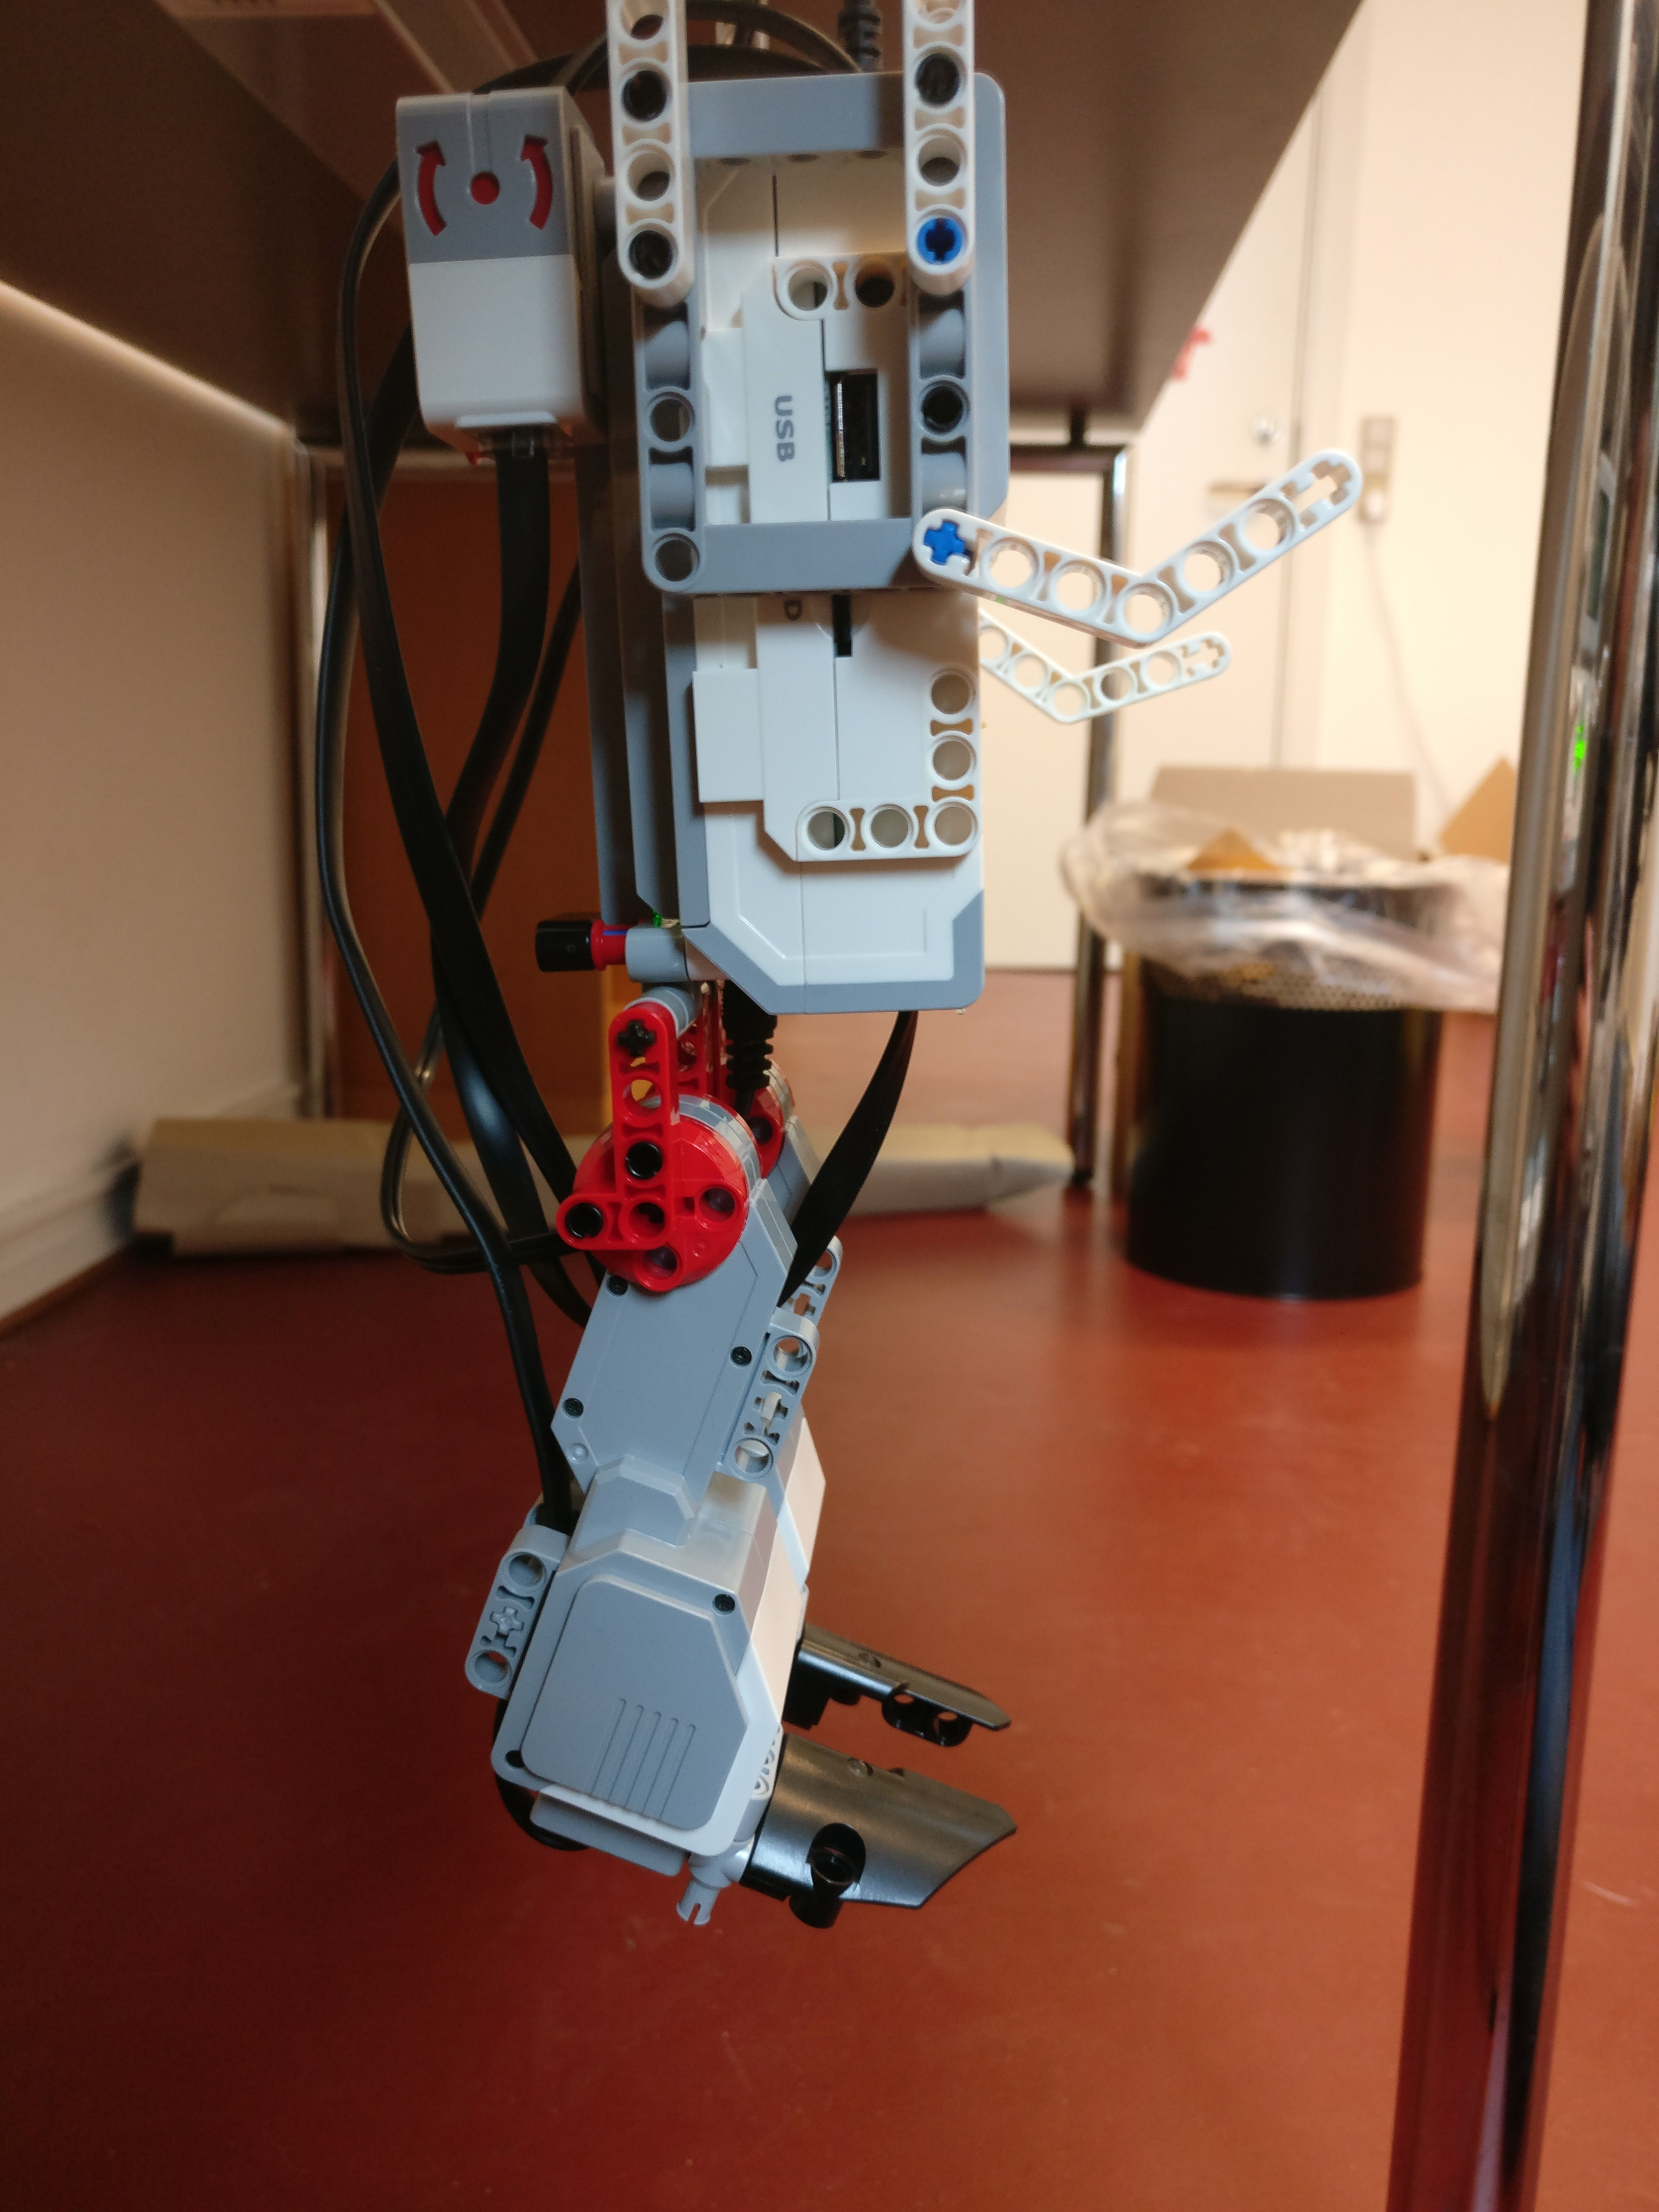
\includegraphics[width=1\linewidth]{images/swing_robot_side_right}
			\caption{Swing robot, side view. Here the gyroscope is visible in the top left.}
			\label{fig:swing_robot_side}
		\end{subfigure}%
		\caption{Swing robot design. The corpus is hanging on a harness and can freely rotate around the mount at the top of the frame. A gyroscope is mounted on the back of the robot.}
		\label{fig:swing_robot}
	\end{figure}
	
	To be able to swing, the robot must move some amount of counterweight, this is achieved by having each "leg" consisting of a large motor mounted backwards, such that the big and heavy part of the motor is moved. See Figure \ref{fig:swing_robot_side} for a view of the leg. To reduce training complexity, the legs are physically attached to each other, and moved as one. This has the added benefit of significantly reducing the time required to move both legs, allowing us to take actions at a higher frequency and also solved an issue of the legs not moving completely synchronous due to slight delays.
	
	To observe the swinging motion, a gyroscope is mounted at the back of the robot.The height of the gyroscope was chosen to provide the most stable observations and the least drift in angle over time. The gyroscope measures angle and rate of the robot \footnote{see section \ref{gyro_section}}. Combining angle and rate with the position of the legs should be all the information needed to describe the robot at a given point in time, eliminating the need to make the system recurrent or otherwise including information about past points in time. Eliminating this need should make learning easier.
	
	To provide a solid mount for the swing, the horizontal bar of rotation is firmly attached to two tables, as shown in Figure \ref{fig:swing_robot_front}. This proved to be very stable. While a table mount is a very available solution, as tables are abundant in most educational facilities, it does obstruct the visibility of the demonstration. For demonstration purposes it would be better to have less visually obstructive frame. We experimented with a frame build out of LEGO, but this requires a lot of LEGO bricks and is not very solid. An alternative is a metal frame, which we plan to construct later on.
	
	To control the robots basic functions, such as moving the legs and reading sensor data, we implemented a robot control class \footnote{The robot controller is available on github in the file \texttt{src/swing\_robot/robot\_controler.ipynb}.}. It offers a high level interface that can be used for learning.
	
	\subsection{Formulation of the Learning Problem}
	In this section we discuss how to structure the problem of teaching the robot how to swing. We start by examining the state and action space defined by the sensors and motors used in the construction of the robot. This leads us to make an decision about what reinforcement learning approaches are feasible for the problem.  Finally we discuss how to define the reward function.
	
	\subsubsection*{State and Action Space}
	To be able to learn how to swing, we need to design the learning problem. To make a decision about what learning approach to use, we first look at the space of inputs and outputs provided by the robot. The information available as a basis for decisions forms the state space $\mathcal{X}$, and is composed of:
	\begin{itemize}
		\item Rate of angle change of the swing. It is measured by the gyro sensor in degrees per second, and is continuous in $\mathbb{R}$. 
		\item Angle of the swing. It is measured by the gyro sensor in degrees, and is continuous in $\mathbb{R}$
		\item Position of the legs. It is measured by the motor in degrees, and is continuous in $\mathbb{R}$
	\end{itemize}
	To facilitate the swing motion, we have to move the legs of the robot. This defines the action space $\mathcal{Y}$, and is the output of our prediction process:
	\begin{itemize}
		\item Position to move the legs to. The motors can be instructed to move to an angle in degrees. The space is continuous in $\mathbb{R}$.
	\end{itemize}
	
	
	\subsubsection*{Reinforcement Learning Approach}
	As both $\mathcal{X}$ and $\mathcal{Y}$ are continuous, we can not use the Q-learning approach used in the crawl robot. For the crawl robot, the arm would always be in a predetermined set of positions, where even if we made the action space discrete for the swing, the input space would still be continuous. 
	Instead, we need a reinforcement learning algorithm that can handle both continuous state and action spaces. Such a function, mapping from a continuous space to another of different dimension, can be approximated by a neural network. A neural network performs a prediction by forward feeding the inputs through its layers. It learns by comparing it's prediction to the true label and updates its weights with back propagation. However, we do not know the true label, which in this case would be the optimal movement of the legs, and can thus not use back propagation to update the neural networks weights. We need a different approach to learning.
	
	A common way of using neural networks in reinforcement learning is to couple them with the Covariance Matrix Adaptation Evolution Strategy (CMA-ES). CMA-ES is regarded as the state of the art in evolutionary and numerical optimization \cite{beyer}\cite{eiben_smith_2015}, for optimization problems in an unconstrained continuous space when no gradients are available. In this set up, the neural network is used as a function approximator. Each function approximator is evaluated, and scored with a reward function. CMA-ES is used to test different weights for the neural network, and based on the evaluation of each set of weights, it is able to optimize the weights for the neural network, and thus finding an optimal function approximator.
	
	\begin{figure}[h]
		\centering
		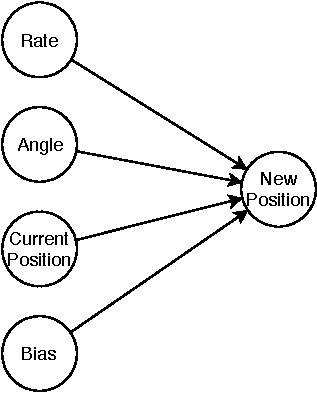
\includegraphics[width=0.3\linewidth]{images/swing_NN.pdf}
		\caption{The perceptron (linear Neural Network) used as a function approximator for the swing.}
		\label{fig:swing_NN}
	\end{figure}
	
	\subsubsection*{Function Approximator}
	For our particular learning problem we use a linear neural network (also called perceptron) as the function approximator. This results in the neural network having few weights, which reduces training time and allows us to analyze the result by looking at individual weights. The symmetric nature of the swinging movement let us to experiment with removing the bias term, however we noticed that the bias is very important to allow the swing to move out of the initial resting position, where all three inputs are $0$. 
	
	To ensure that all predictions will be valid positions that we can move the motors to, we normalize all inputs and outputs to a $[-1, 1]$ interval, and select $\tanh(x)$ as the activation function. This leads to the formal definition of the function approximator as
	$$
	y = \tanh{ \bigg( \sum_{i=1}^3 w_i x_i + b \bigg) }
	$$
	where $y$ is the position to move the legs to, $w_i$ is the weight for input $x_i$ and $b$ the bias. CMA-ES optimizes 4 dimensions: $w_1, w_2, w_3, b$.
	
	\subsubsection*{Evaluation of the Function Approximator}
	To evaluate a choice of weights for the function approximator, we run a trial run of it on the swing. Each trial starts with the swing hanging at an angle of $0$ degrees. In this position it is motionless, thus having a rate of $0$ degrees per second. The legs are in the default position $0$. During the trial we repeatedly execute three steps in a loop:
	\begin{enumerate}
		\item Take measurements of the inputs $x_1, x_2, x_3$
		\item Calculate the prediction $y$ based on the inputs with the function approximator.
		\item Move the legs to position $y$.
	\end{enumerate}
	Each trial run lasts for 30 seconds. This gives the robot plenty of time to start swinging. After the trial period we move the legs back into the initial position and wait for the swing to come to a standstill. The standstill is determined by the gyro sensor rate measurement being constant over a three second time-frame. If the angle or rate measurements at standstill are different from $0$, we automatically re-calibrate the gyro sensor.
	
	The reward is calculated based on the maximum absolute rate measured during the trial. We believe this is a good and robust quantifier for how good the swinging motion is. Other options, such as the highest measured absolute angle would be good alternatives.
	
	
	\begin{figure}[ht]
		%\centering
		\raggedright
		\begin{subfigure}{.48\textwidth}
			\centering
			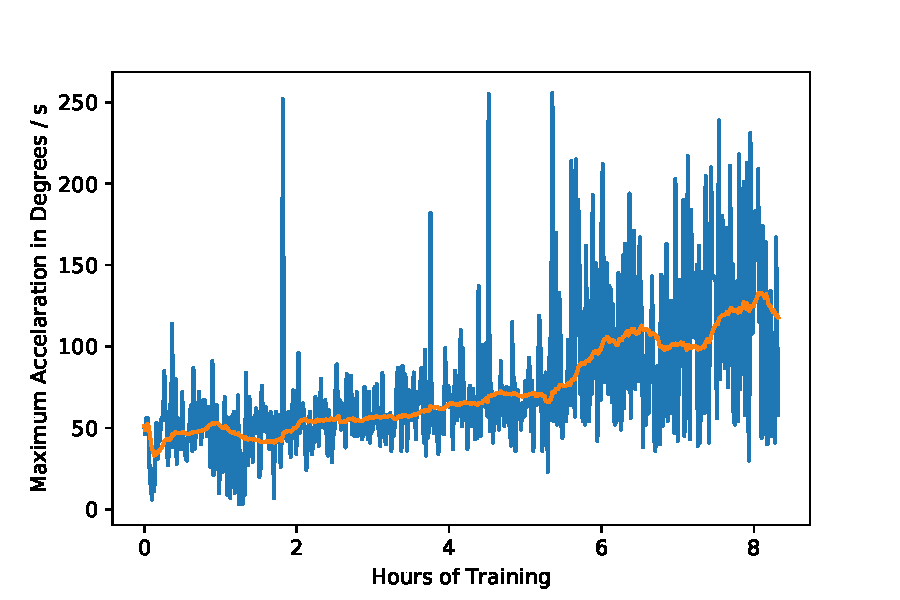
\includegraphics[width=1\linewidth]{images/swing_rewards}
			\caption{Reward of function approximator evaluations during training. Orange represents the rolling average over 50 data-points. A clear improvement is visible.}
			\label{fig:swing_rewards}
		\end{subfigure}
		\begin{subfigure}{.48\textwidth}
			\centering
			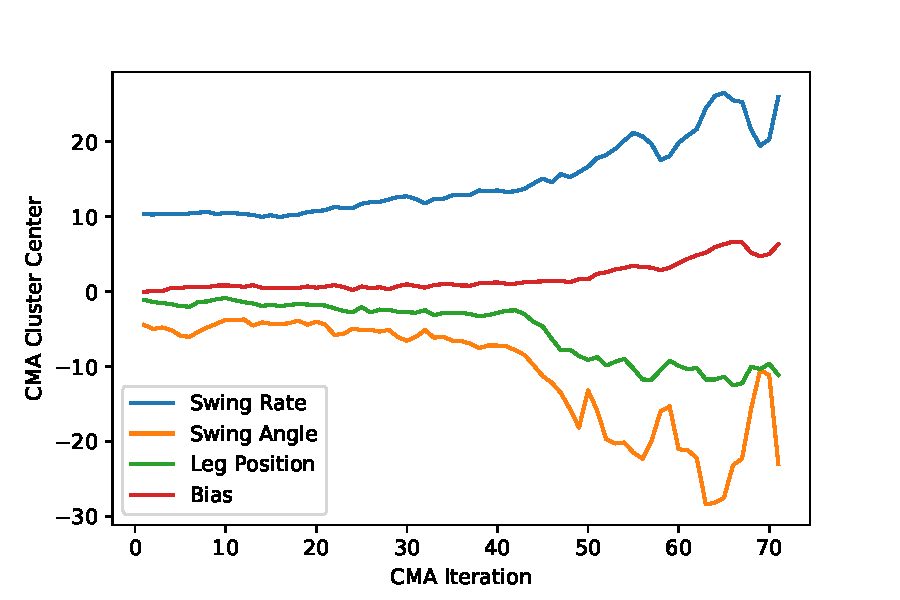
\includegraphics[width=1\linewidth]{images/swing_weights}
			\caption{Development of the weights of the CMA mean during training.}
			\label{fig:swing_weights}
		\end{subfigure}
		\begin{subfigure}{.48\textwidth}
			\centering
			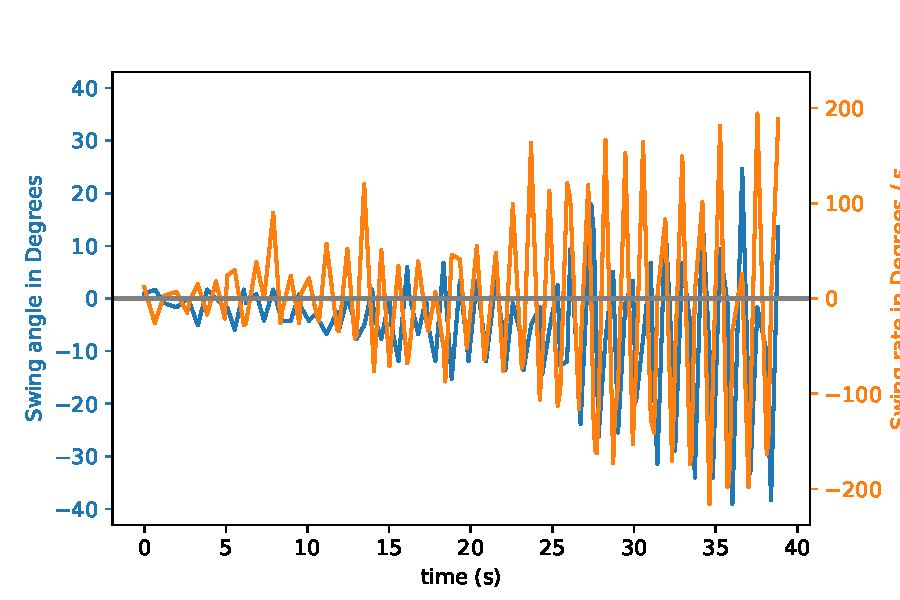
\includegraphics[width=1\linewidth]{images/trail_run.pdf}
			\caption{Measurements of rate and angle of the optimal model during a trial run..}
			\label{fig:swing_plot}
		\end{subfigure}%
		\caption{Development of rewards and weights during training of the swing.}
		\label{fig:swing_results}
	\end{figure}
	
	\subsection{Swing robot results}
	The training is initialized with 'best guess' weights, which assign the small bias of $0.2$ to start moving the legs, a large weight of $10$ for the rate to move legs in the direction of the current movement, a negative weight of $-5$ for the angle to move legs less drastically in a direction when already on that side, and $-1$ to the previous leg position to force some movement of the legs even if nothing else is happening in the system. With the initial parameter choices, a maximum rate of 56 degrees / second was measured. 
	
	From these best guess initial parameter choices, the CMA-ES optimizer is set to train. After 8h 20min of training the robots battery was depleted, marking the end of training. The CMA-ES optimizer performed a total of 568 function evaluations over 71 CMA-ES iterations. The final model achieved a maximum rate of 256 degrees / second, which is a 5 times improvement over the initial choices. The training progress is shown in Figure \ref{fig:swing_results} and has been posted online\footnote{Available at \url{https://youtu.be/6yY9P5vG-nA}.}. We can observe that the maximum acceleration measured increases during training, indicating that the learning was successful. A significant increase in the rewards attained is visible around the 5 hour mark, afterwards the rewards seem to plateau. Furthermore we note that the plot is very noisy, indicating that the experiment is unstable, or the function we try to learn very non-smooth.
	
	The development of the CMA-ES weights is visualized in Figure \ref{fig:swing_weights}. Over the training duration, all 4 weights shifted significantly. Coinciding with the big increase in reward around the 5 hour mark, we see large movements in the weights around this time as well. It appears that our initial guesses were pretty good, as the order of the magnitudes of the parameter choices at the end of training is identical to our initialization. 
	
	Measurements taken during a trial run the the optimal weights is shown in Figure \ref{fig:swing_plot}. We can see that the robot slowly ramps up, an reaches the maximum amplitude after about 30 seconds.
	
	
	\subsection{Swing robot discussion}
	A robot can be aiding the educational process and scientific outreach in different ways. A training time of over five hours to get noticeable results, and more than eight hours until training is complete does hinder its use in a traditional classroom settings where students observe the entire learning process. However, we want to highlight the potential use of the swing as a demonstration object. The robot trained independently for more than eight hours, and would have trained even longer if the battery did not run out. This is a testament of the reliability of the software and hardware developed, and allows for much longer training than would be feasible for robots that need more supervision and interaction. It makes this robot an ideal presentation piece that can run for hours or even days at a science exhibition. The impressive nature of the swinging motion helps to raise interest in the robot, and by extension the machine learning and robotics used to create it. Compared to the two previous robots presented, the swing robot offers an interactive experience not during training, but in the trained swinging motion itself. People can push and pull on the swinging robot, and observe how the robots interacts to these outward influence.
	
	\medskip
	
	Based on the development of the weights, shown in Figure \ref{fig:swing_weights}, it is possible to interpret what influences an ideal swinging motion. By looking at the weights, we kan see that leg position is strongly influenced by the direction of the current movement (eg: if moving forward, move your legs forward), and opposite of the current swing angle (eg: if very far forward, start moving your legs back). The position is less heavy influenced by the current leg position (eg: if your legs are forward, start moving them back), and only slightly influenced by the bias term (eg: if standing still, move your legs forward). 
	
	\medskip
	
	When observing the robot swinging, it is apparent that the leg movements are not smooth, and appear abrupt at some points. This behaviour is captured in Figure \ref{fig:swing_plot}, where the rate and angle measurements taken during the trial run are shown. We attribute this behaviour to the low sample rate of the robot. During execution of the trained motion, each iteration of the main execution loop, consisting of taking a sample and moving the legs accordingly, took on average 0.35 seconds, resulting in a sample rate of 2.8Hz. To attain a smoother motion and faster reactions, the sample rate has to be increased. Profiling the current Python implementation did not reveal any possible significant performance gains. We believe that to attain significantly faster response times, the program would have to be implemented in a faster, more low level language.
	
	\medskip
	The swing motion could further improved by testing different reinforcement learning architectures. We selected a simple linear neural network to reduce the complexity and thus the learning time. But as the robot proved to be highly autonomous and can train for long time spans without supervision, more complex models could be used. The related models of neural networks with hidden neurons, and recurrent neural networks are potential candidates that should be evaluated. It is also possible to move each leg individually, which could be further explored.
	
	
	
	\section{Results}
	A colour detection robot has been created, representing the simplest level of complexity, with a focus on visualization and education. Two forms of KNN have been implemented for the colour robot, as well as a neural network. Forms of visualization have been explored and implemented, see for example Figure \ref{fig:colour_KNN_binary}.
	\medskip
	
	A crawling robot has been created, representing the middle level of complexity of our robots, with a balanced combination of task complexity and educational accessibility. The crawling robot learns a crawling motion almost to perfection after about 20 minutes of training. It learns using tabular Q-learning, and a video of said training has been posted\footnote{Available at \url{https://youtu.be/NUTv-oNWEYo}.}.
	\medskip
	
	A swing robot has been created, representing the highest level of complexity of our robots, suitable as for example a presentation piece. The swing robot predicts leg movements using a simple perceptron, and CMA-ES was implemented for training it. It learned a swinging motion over eight hours on unsupervised training, reaching most of its potential after about five hours of training, and a video of it has been posted\footnote{Available at \url{https://youtu.be/6yY9P5vG-nA}.}. 
	\medskip
	
	We have created a diverse set of robots that complete different tasks using different learning algorithms, and have documented this using pictures, videos, plots and other forms of visual aids. The robots cover a wide range of complexities and offer different educational opportunities. Future developments of each type of robot has been discussed, covering wide ranges of mathematical and practical difficulty levels.
	
	\section{Discussion}
	It is our goal to explore ways of explaining machine learning concepts with educational aids. Decision boundaries are a good tool to visualize the prediction process and the colour robot appeared to be the best candidate for this, with a focus on visualization. Unfortunately, it was not possible to reduce the three dimensional colour data to two dimensions in an easily understandable way, and we found no suitable approach to visualize a decision boundary in higher dimensions. A good candidate for future development would be implementing an evolving decision boundary for a KNN or similar system, that pupils can interact with, to see the boundary change with new observations.
	\medskip
	
	When working with pupils, capturing their energy and excitement is important. Lessons should be short and engaging. If the training takes too long, students can lose interest. Thus the training process of a robot should be kept to a minimum, so we designed the crawl robot with this in mind. By simplifying the learning process, we are able to reduce the training time to 20 minutes. This training process is short and highly interactive, as students can observe the robot getting better and have to repeatably move it back to its starting position. We think this robot can serve as a good representation of the training process, which is an essential part of machine learning.
	\medskip
	
	The swing robot is a big and imposing robot, that showcases what is possible with reinforcement learning. With a training time of over eight hours makes it impractical for classroom settings, but can serve as a presentation piece at exhibitions or science museums. While not interactive during training, the trained model can be set to run in an infinite loop to show what is possible to achieve with reinforcement learning. It is also fun to poke the swinging robot and observe how it reacts to these adversarial intrusions.
	
	\medskip 
	
	\subsubsection*{Lessons Learned} 
	From designing these projects, we learned the importance of considering from the start how automated the training can be made. The swing needs to train for five to eight hours, which is only practically possible because it doesn't need human interaction during training. The crawling robot needs a lot of interaction to reset it and keep it aligned, which limits the practically feasible training time considerably, as both pupils and researchers patience is limited. A well designed robot needs to balance training time and necessary supervision.
	
	Another discussion point for every future robot will be how to design the action space. For our crawl robot, we use a discrete action space, while the swing robot uses a continuous action space. Sometimes, one option will be obviously more fit to the problem than the other, but there exists a trade-off between training speed, where discrete options train slightly faster, and smoothness, where a continuous action space creates smoother movement.
	
	Finally, in an educational setting, it is important to consider how the robot aids learning and understanding of machine learning. We present robots that demonstrate the learning process, as well as robots where the final result is more interesting. In some robots students can follow the learning graphically, while others present results as a physical movement. Some robots are big and inspiring, which can be utilized to attract an audience, while others work better with small groups that spent an extended amount of time working on the robot. We demonstrated examples encompassing a broad range of complexity, availability, interests, and use cases.
	
	\subsection{Future Work}
	This project has sparked some new ideas for how the LEGO Mindstorms robots can be used for future projects, for both specific robots designed to learn specific tasks, and more overall subjects to work on.
	
	Early on in the project, we learned that some robots shared publicly used faster motors and more accurate sensors available from third party providers\footnote{A third party provider manufacturing custom sensors and motors compatible with LEGO Mindstorms is \texttt{http://www.mindsensors.com/}.}. For this project, we decided to use stock LEGO parts only, but a possible future topic could be the usage of custom hardware. This would probably make the existing robots more accurate, and may open up robots that require faster reaction times, such as the pole balancing robot seen in \cite{youtube_pole}.
	
	In a common classroom setting there are multiple groups of students working on building and operating the same robot model individually. This inspired the idea that multiple robots training on the same task can share knowledge to train faster. This is called multi-actor learning, and has the potential of speeding up training times in the classroom, thus reducing down time and enabling the project to fit into a typical time slot in school schedules.
	
	With the LEGO Mindstorms platform, the central processing component can be used for many different tasks. LEGO may be interested in implementing multi-purpose solutions for their distributions, which utilize a graphical programming language. For our robots, we implemented a tailor made solution in Python for the specific problem. Bridging this gap from a specialized prototype to a multi purpose commercial product does require further development. Google's Atari bot from 2013 achieved high performance on seven different games, using the same learning system \cite{google_deepmind_atari}. It may be interesting to offer the algorithms used in this project as a general module that can learn in different robot and task configurations. It could also be interesting to study modular robots, with varying amounts of motors and/or sensors.
	
	
	\section{Individual contributions}
	This project is a joint effort of the two authors. The colour robot was exclusively worked on by Asger Hans Skovbjerg Christensen, while the crawl robot is the exclusive work of Per Steffen Czolbe. All other robots and report sections are the product of both authors work.
	
	
	\bibliographystyle{abbrv}
	\bibliography{references}
	
\end{document}
